% Options for packages loaded elsewhere
\PassOptionsToPackage{unicode}{hyperref}
\PassOptionsToPackage{hyphens}{url}
%
\documentclass[
]{book}
\usepackage{amsmath,amssymb}
\usepackage{iftex}
\ifPDFTeX
  \usepackage[T1]{fontenc}
  \usepackage[utf8]{inputenc}
  \usepackage{textcomp} % provide euro and other symbols
\else % if luatex or xetex
  \usepackage{unicode-math} % this also loads fontspec
  \defaultfontfeatures{Scale=MatchLowercase}
  \defaultfontfeatures[\rmfamily]{Ligatures=TeX,Scale=1}
\fi
\usepackage{lmodern}
\ifPDFTeX\else
  % xetex/luatex font selection
\fi
% Use upquote if available, for straight quotes in verbatim environments
\IfFileExists{upquote.sty}{\usepackage{upquote}}{}
\IfFileExists{microtype.sty}{% use microtype if available
  \usepackage[]{microtype}
  \UseMicrotypeSet[protrusion]{basicmath} % disable protrusion for tt fonts
}{}
\makeatletter
\@ifundefined{KOMAClassName}{% if non-KOMA class
  \IfFileExists{parskip.sty}{%
    \usepackage{parskip}
  }{% else
    \setlength{\parindent}{0pt}
    \setlength{\parskip}{6pt plus 2pt minus 1pt}}
}{% if KOMA class
  \KOMAoptions{parskip=half}}
\makeatother
\usepackage{xcolor}
\usepackage{longtable,booktabs,array}
\usepackage{calc} % for calculating minipage widths
% Correct order of tables after \paragraph or \subparagraph
\usepackage{etoolbox}
\makeatletter
\patchcmd\longtable{\par}{\if@noskipsec\mbox{}\fi\par}{}{}
\makeatother
% Allow footnotes in longtable head/foot
\IfFileExists{footnotehyper.sty}{\usepackage{footnotehyper}}{\usepackage{footnote}}
\makesavenoteenv{longtable}
\usepackage{graphicx}
\makeatletter
\def\maxwidth{\ifdim\Gin@nat@width>\linewidth\linewidth\else\Gin@nat@width\fi}
\def\maxheight{\ifdim\Gin@nat@height>\textheight\textheight\else\Gin@nat@height\fi}
\makeatother
% Scale images if necessary, so that they will not overflow the page
% margins by default, and it is still possible to overwrite the defaults
% using explicit options in \includegraphics[width, height, ...]{}
\setkeys{Gin}{width=\maxwidth,height=\maxheight,keepaspectratio}
% Set default figure placement to htbp
\makeatletter
\def\fps@figure{htbp}
\makeatother
\setlength{\emergencystretch}{3em} % prevent overfull lines
\providecommand{\tightlist}{%
  \setlength{\itemsep}{0pt}\setlength{\parskip}{0pt}}
\setcounter{secnumdepth}{5}
\usepackage{booktabs}
\ifLuaTeX
  \usepackage{selnolig}  % disable illegal ligatures
\fi
\usepackage[]{natbib}
\bibliographystyle{plainnat}
\IfFileExists{bookmark.sty}{\usepackage{bookmark}}{\usepackage{hyperref}}
\IfFileExists{xurl.sty}{\usepackage{xurl}}{} % add URL line breaks if available
\urlstyle{same}
\hypersetup{
  pdftitle={Topology},
  pdfauthor={Ashan Jayamal},
  hidelinks,
  pdfcreator={LaTeX via pandoc}}

\title{Topology}
\author{Ashan Jayamal}
\date{2024-02-16}

\usepackage{amsthm}
\newtheorem{theorem}{Theorem}[chapter]
\newtheorem{lemma}{Lemma}[chapter]
\newtheorem{corollary}{Corollary}[chapter]
\newtheorem{proposition}{Proposition}[chapter]
\newtheorem{conjecture}{Conjecture}[chapter]
\theoremstyle{definition}
\newtheorem{definition}{Definition}[chapter]
\theoremstyle{definition}
\newtheorem{example}{Example}[chapter]
\theoremstyle{definition}
\newtheorem{exercise}{Exercise}[chapter]
\theoremstyle{definition}
\newtheorem{hypothesis}{Hypothesis}[chapter]
\theoremstyle{remark}
\newtheorem*{remark}{Remark}
\newtheorem*{solution}{Solution}
\begin{document}
\maketitle

{
\setcounter{tocdepth}{1}
\tableofcontents
}
\hypertarget{topology}{%
\chapter{Topology}\label{topology}}

A topology is a geometric structure defined on a set. Basically it is given by declaring which subsets are ``open'' sets. Thus the axioms are the abstraction of the properties that open sets have.

\hypertarget{topological-spaces}{%
\section{Topological Spaces}\label{topological-spaces}}

\begin{definition}
\protect\hypertarget{def:Top}{}\label{def:Top}A topology on a set \(X\) is a collection \(\mathcal{T}\) of subsets of \(X\) such that

(T1) \(\phi\) and \(X\) are in \(\mathcal{T}\);

(T2) Any union of subsets in \(\mathcal{T}\) is in \(\mathcal{T}\);

(T3) The finite intersection of subsets in \(\mathcal{T}\) is in \(\mathcal{T}\).
\end{definition}

A set \(X\) with a topology \(\mathcal{T}\) is called a topological space. Denoted by \((X,\mathcal{T})\). An element of \(\mathcal{T}\) is called an open set.

\begin{example}
\protect\hypertarget{exm:unnamed-chunk-1}{}\label{exm:unnamed-chunk-1}Let \(X\) be a three-element set, \(X = \{a, b, c\}\) and \(\mathcal{T}=\{X, \emptyset,\{a, b\}, \{b\}, \{b, c\}\}\). We can check T1,T2 and T3 conditions.
\end{example}

\begin{example}
\protect\hypertarget{exm:unnamed-chunk-2}{}\label{exm:unnamed-chunk-2}Let \(X\) be a three-element set, \(X = \{a, b, c\}\) as pervoius. There are many possible topologies on \(X\), some of which are indicated schematically in figure \ref{fig:gi}. Furthur, we can see that even a three-element set has many different topologies.
\end{example}

\begin{figure}
\centering
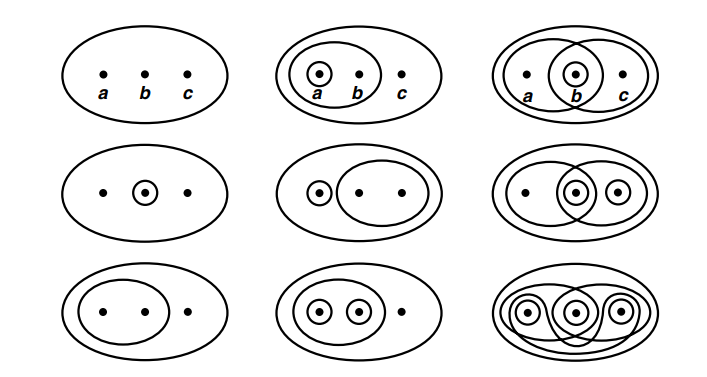
\includegraphics{figures/figure 01.png}
\caption{\label{fig:gi}\(~\)}
\end{figure}

\begin{remark}
Not every collection of subsets of \(X\) is a topology on \(X\). Observe that Neither of the collections indicated in figure \ref{fig:fig2} is a topology.

First let's consider the left hand coner of figure \ref{fig:fig2}. \(\{a\}\) and \(\{b\}\) in the collection, but \(\{a\}\cup \{b\}\) is not in the collection.

Now consider the right hand coner figure. \(\{a,b\}\) and \(\{b,c\}\) in collection, but \(\{a,b\}\cap\{b,c\}=\{b\}\) is not in the collection.
\end{remark}

\begin{figure}
\centering
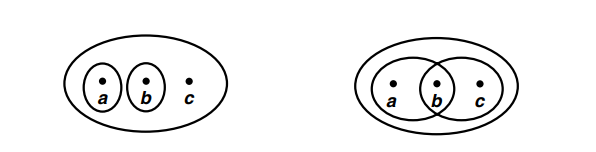
\includegraphics{figures/figure 02.png}
\caption{\label{fig:fig2}\(~\)}
\end{figure}

\begin{example}
\protect\hypertarget{exm:unnamed-chunk-4}{}\label{exm:unnamed-chunk-4}If \(X\) is any set, the collection of all subsets of \(X\) (Power set) is a topology on \(X\). This trivail statified T1 T2 and T3 conditions. Furthur,This is called the \emph{discrete topology}.
\end{example}

\begin{example}
\protect\hypertarget{exm:unnamed-chunk-5}{}\label{exm:unnamed-chunk-5}The collection consisting of \(X\) and \(\emptyset\) only is also a topologyon \(X\). we shall call it the \emph{indiscrete topology}, or the trivial topology.
\end{example}

\begin{example}
\protect\hypertarget{exm:unnamed-chunk-6}{}\label{exm:unnamed-chunk-6}Let \(X\) be a set and let \(\mathcal{T}_f\) be the collection of all subsets U of X such that \(X\setminus U\) either is finite or is all of \(X\). In oter words,
\[\mathcal{T}_f:=\left\{U\subseteq X : \text{Either is finite or is all of } X\right\}\]
Let's check is \(\mathcal{T}_f\) a topology. First obseve that both \(X\) and \(\emptyset\) are in \(\mathcal{T}_f\) , because \(X\setminus X=\emptyset\) is finite and \$X\setminus \emptyset \$ is all of \(X\).So \(\mathcal{T}_f\) statified the T1 condition. Now let's check the T2 condition. Let \(\{U_{\alpha}:\alpha\in I, I \text{ is index set}\}\).Now we need to show that \(\cup{\alpha\in I} U_\alpha\in \mathcal{T}_f\). So consider,
\[X\setminus \bigcup_{\alpha\in I} U_\alpha =\bigcap_{\alpha\in I} (X\setminus  U_\alpha).\]
Now obsevere that \(\cap_{\alpha\in I} (X\setminus U_\alpha)\) is finite, because each set \((X\setminus U_\alpha)\) is finite and arbitary intersection of finite sets is finite. So, \(\mathcal{T}_f\) stattified the T2 condition also.
Finaly check the last condition, T3 condition. Let \(U_1,...,U_n\) are nonempty elements of \(\mathcal{T}_f\) , to show that \(\bigcup_i U_i \in \mathcal{T}_f\) , we compute
\[X\setminus \bigcap_{i=1}^n U_i = \bigcup_{i=1}^n(X \setminus U_i).\]
Note that the set \(\bigcup_{i=1}^n(X \setminus U_i)\) is a finite union of finite sets and, therefore, finite. So it statisfiy the T3 condition also. Thefore \(\mathcal{T}_f\) is a topology. Furthur \(\mathcal{T}_f\) is called the finite \emph{complement topology}.
\end{example}

\begin{example}
\protect\hypertarget{exm:unnamed-chunk-7}{}\label{exm:unnamed-chunk-7}Let \(X\) be a set. Define \(\mathcal{T}\) to be the collection of all subsets \(U\) of \(X\) such that \(X\setminus U\) either is finite or is all of \(X\). Then \(\mathcal{T}\) defines a topology on \(X\), called finite complement topology of \(X\).
\end{example}

\hypertarget{basis-of-a-topology}{%
\section{Basis of a Topology}\label{basis-of-a-topology}}

Once we define a structure on a set, often we try to understand what the minimum data you need to specify the structure. In many cases, this minimum data is called a basis and we say that the basis generate the structure. The notion of a basis of the structure will help us to describe examples more systematically.

\begin{definition}
\protect\hypertarget{def:unnamed-chunk-8}{}\label{def:unnamed-chunk-8}Let \(X\) be a set. A basis of a topology on \(X\) is a collection \(\mathcal{B}\) of subsets in \(X\) such that

(B1) For every \(x \in X\), there exist an element \(B\) in \(\mathcal{B}\) such that \(x \in B\).

(B2) If \(x \in B_{1} \cap B_{2}\) where \(B_{1}, B_{2}\) are in \(\mathcal{B}\), then there is \(B_{3}\) in \(\mathcal{B}\) such that \(x \in B_{3} \subseteq B_{1} \cap B_{2}\).
\end{definition}

\begin{figure}
\centering
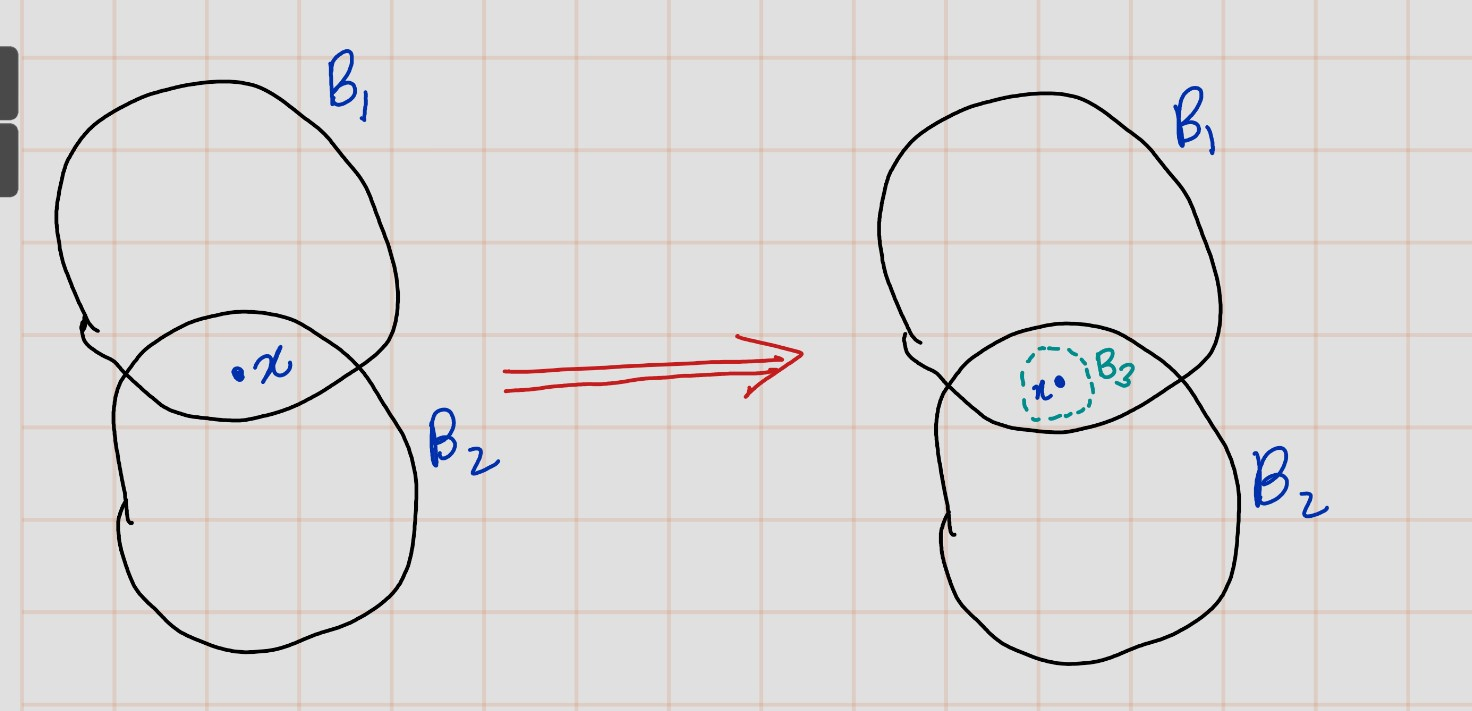
\includegraphics{figures/figure 03.jpg}
\caption{\label{fig:fig3}\(~\)}
\end{figure}

\begin{lemma}[Generating of a topology]
\protect\hypertarget{lem:unnamed-chunk-9}{}\label{lem:unnamed-chunk-9}Let \(\mathcal{B}\) be a basis of a topology on X. Define \(\mathcal{T}_{\mathcal{B}}\) to be the collection of subsets \(U \subset X\) satisfting

(G1) For every \(x \in U\), there is \(B \in \mathcal{B}\) such that \(x \in B \subset U\).

Then \(\mathcal{T}_{\mathcal{B}}\) defines a topology on \(X\). Here we assume that \(\emptyset\) trivially satisfies the condition, so that \(\emptyset \in \mathcal{T}_{\mathcal{B}}\).
\end{lemma}

\begin{proof}

We need to check the three axioms:

\begin{itemize}
\item
  (T1) \(\emptyset \in \mathcal{T}_{\mathcal{B}}\) as we assumed. \(X \in \mathcal{T}_{\mathcal{B}}\) by (B1).
\item
  (T2) Consider a collection of subsets \(U_{\alpha} \in \mathcal{T}_{\mathcal{B}}, \alpha \in \mathrm{J}\). We need to show
\end{itemize}

\[
U:=\bigcup_{\alpha \in J} U_{\alpha} \quad \in \mathcal{T}_{\mathcal{B}}
\]
By the definition of the union, for each \(x \in U\), there is \(U_{\alpha}\) such that \(x \in U_{\alpha}\). Since \(U_{\alpha} \in \mathcal{T}_{\mathcal{B}}\), there is \(B \in \mathcal{B}\) such that \(x \in B \subset U_{\alpha}\). Since \(U_{\alpha} \subset U\), we found \(B \in \mathcal{B}\) such that \(x \in B \subset U\). Thus \(U \in \mathcal{T}_{\mathcal{B}}\).

\begin{itemize}
\item
  (T3) Now consider a finite number of subsets \(U_{1},..., U_{n} \in \mathcal{T}_{\mathcal{B}}\). We need to show that
  \[
  U':=\bigcap_{i=1}^{n} U_{i} \quad \in \mathcal{T}_{\mathcal{B}}
  \]
\item
  Let's just check for two subsets \(U_{1}, U_{2}\) first. For each \(x \in U_{1} \cap U_{2}\), there are \(B_{1}, B_{2} \in \mathcal{B}\) such that \(x \in B_{1} \subset U_{1}\) and \(x \in B_{2} \subset U_{2}\). This is because \(U_{1}, U_{2} \in \mathcal{T}_{\mathcal{B}}\) and \(x \in U_{1}, x \in U_{2}\). By (B2), there is \(B_{3} \in \mathcal{B}\) such that \(x \in B_{3} \subset B_{1} \cap B_{2}\). Now we found \(B_{3} \in \mathcal{B}\) such that \(x \in B_{3} \subset U\).
\item
  We can generalize the above proof to \(n\) subsets, but let's use induction to prove it. This is going to be the induction on the number of subsets.

  \begin{itemize}
  \tightlist
  \item
    When \(n=1\), the claim is trivial.
  \item
    Suppose that the claim is true when we have \(n-1\) subsets, i.e.~\(U_{1} \cap \cdots \cap U_{n-1} \in \mathcal{T}_{\mathcal{B}}\). Since \[
    U=U_{1} \cap \cdots \cap U_{n}=\left(U_{1} \cap \cdots \cap U_{n-1}\right) \cap U_{n}
    \]
    and regarding \(U^{\prime}:=U_{1} \cap \cdots \cap U_{n-1}\), we have two subsets case \(U=U^{\prime} \cap U_{n}\). By the first arguments, \(U \in \mathcal{T}_{\mathcal{B}}\).
  \end{itemize}
\end{itemize}

\end{proof}

\begin{definition}
\protect\hypertarget{def:unnamed-chunk-11}{}\label{def:unnamed-chunk-11}\(\mathcal{T}_{\mathcal{B}}\) is called the \textbf{topology generated by a basis \(\mathcal{B}\)}. On the other hand, if \((X, \mathcal{T})\) is a topological space and \(\mathcal{B}\) is a basis of a topology such that \(\mathcal{T}_{\mathcal{B}}=\mathcal{T}\), then we say \(\mathcal{B}\) is a basis of \(\mathcal{T}\). Note that \(\mathcal{T}\) itself is a basis of the topology \(\mathcal{T}\). So there is always a basis for a given topology.
\end{definition}

\begin{example}
\protect\hypertarget{exm:unnamed-chunk-12}{}\label{exm:unnamed-chunk-12}\leavevmode

\begin{itemize}
\item
  (Standard Topology of \(\mathbb{R}\) ) Let \(\mathbb{R}\) be the set of all real numbers. Let \(\mathcal{B}\) be the collection of all open intervals:
  \[
  (a, b):=\{x \in \mathbb{R} \mid a<x<b\}
  \]
  Then \(\mathcal{B}\) is a basis of a topology and the topology generated by \(\mathcal{B}\) is called the standard topology of \(\mathbb{R}\).
\item
  Let \(\mathbb{R}^{2}\) be the set of all ordered pairs of real numbers, i.e.~\(\mathbb{R}^{2}:=\mathbb{R} \times \mathbb{R}\) (cartesian product). Let \(\mathcal{B}\) be the collection of cartesian product of open intervals, \((a, b) \times(c, d)\). Then \(\mathcal{B}\) is a basis of a topology and the topology generated by \(\mathcal{B}\) is called the standard topology of \(\mathbb{R}^{2}\).
\item
  (Lower limit topology of \(\mathbb{R}\) ) Consider the collection \(\mathcal{B}\) of subsets in \(\mathbb{R}\) :
  \[
  \mathcal{B}:=\{[a, b):=\{x \in \mathbb{R} \mid a \leq x<b\} \mid a, b \in \mathbb{R}\}
  \]
  This is a basis for a topology on \(\mathbb{R}\). This topology is called the lower limit topology.
\end{itemize}

\end{example}

The following two lemma are useful to determine whehter a collection \(\mathcal{B}\) of open sets in \(\mathcal{T}\) is a basis for \(\mathcal{T}\) or not.

\begin{remark}
Let \(\mathcal{T}\) be a topology on \(X\). If \(\mathcal{B} \subset \mathcal{T}\) and \(\mathcal{B}\) satisfies (B1) and (B2), it is easy to see that \(\mathcal{T}_{\mathcal{B}} \subset \mathcal{T}\). This is just because of (G1). If \(U \in \mathcal{T}_{\mathcal{B}}\), (G1) is satisfied for \(U\) so that \(\forall x \in U, \exists B_{x} \in \mathcal{B}\) such that \(x \in B_{x} \subset U\). Therefore \(U=\cup_{x \in U} B_{x}\). By (T2), \(U \in \mathcal{T}\).
\end{remark}

\begin{lemma}
\protect\hypertarget{lem:lemmaTequalsTB}{}\label{lem:lemmaTequalsTB}Let \((X, \mathcal{T})\) be a topological space. Let \(\mathcal{B} \subset \mathcal{T}\). Then \(\mathcal{B}\) is a basis and \(\mathcal{T}_{\mathcal{B}}=\mathcal{T}\) if and only if \(\mathcal{T}\) is the set of all unions of elements in \(\mathcal{B}\).
\end{lemma}

\begin{proof}
\leavevmode

\begin{itemize}
\tightlist
\item
  \(\quad(\Rightarrow)\) Let \(\mathcal{T}^{\prime}\) be the set of all unions of open sets in \(\mathcal{B}\). If \(U \in \mathcal{T}\), then \(U\) satisfies (G1), i.e.~\(\forall x \in U, \exists B_{x} \in \mathcal{B}\) s.t. \(x \in B_{x} \subset U\). Thus \(U=\cup_{x \in U} B_{x}\). Therefore \(U \in \mathcal{T}^{\prime}\). We proved \(\mathcal{T} \subset \mathcal{T}^{\prime}\). It follows from (T2) that \(\mathcal{T}^{\prime} \subset \mathcal{T}\).
\item
  \((\Leftarrow)\) Since \(X \in \mathcal{T}, X=\cup_{\alpha} B_{\alpha}\) some union of sets in \(\mathcal{B}\). Thus \(\forall x \in X, \exists B_{\alpha}\) s.t. \(x \in B_{\alpha}\). This proves (B1) for \(\mathcal{B}\). If \(B_{1}, B_{2} \in \mathcal{B}\), then \(B_{1} \cap B_{2} \in \mathcal{T}\) by (T2). Thus \(B_{1} \cap B_{2}=\cup_{\alpha} B_{\alpha}, B_{\alpha} \in \mathcal{B}\). So \(\forall x \in B_{1} \cap B_{2}, \exists B_{\alpha} \in B\) s.t. \(x \in B_{\alpha}\). This \(B_{\alpha}\) plays the role of \(B_{3}\) in (B2). Thus \(\mathcal{B}\) is a basis. Now it makes sense to consider \(\mathcal{T}_{\mathcal{B}}\) and we need to show \(\mathcal{T}_{\mathcal{B}}=\mathcal{T}\). By the remark, we already know that \(\mathcal{T}_{\mathcal{B}} \subset \mathcal{T}\). On the other hand, if \(U \in \mathcal{T}\), then \(U=\cup_{\alpha} B_{\alpha}, B_{\alpha} \in \mathcal{B}\). Hence, \(\forall x \in U, \exists B_{\alpha}\) such that \(x \in B_{\alpha} \subset U\). Thus (G1) is satisfied for \(U\). Thus \(U \in \mathcal{T}_{\mathcal{B}}\). This proves \(\mathcal{T}_{\mathcal{B}} \supset \mathcal{T}\).
\end{itemize}

\end{proof}

\begin{lemma}
\protect\hypertarget{lem:lemma110}{}\label{lem:lemma110}Let \((X, \mathcal{T})\) be a topological space. Let \(\mathcal{B} \subset \mathcal{T}\). Then \(\mathcal{B}\) is a basis and \(\mathcal{T}_{\mathcal{B}}=\mathcal{T}\) if and if any \(U \in \mathcal{T}\) satisfies (Gl), i.e.~\(\forall x \in U, \exists B_{x} \in \mathcal{B}\) s.t. \(x \in B_{x} \subset U\).
\end{lemma}

\begin{proof}
\leavevmode

\begin{itemize}
\item
  (\(\Rightarrow\)) Trivial by the definition of \(\mathcal{T}_{\mathcal{B}}\).
\item
  (\(\Leftarrow X\)) satisfies (G1) so \(\mathcal{B}\) satisfies (B1). Let \(B_{1}, B_{2} \in \mathcal{B} \subset \mathcal{T}\). By (T3), \(B_{1} \cap B_{2} \in \mathcal{T}\). Thus \(B_{1} \cap B_{2}\) satisfies (G1). This means (B2) holds for \(\mathcal{B}\). Thus \(\mathcal{B}\) is a basis. Now the assumption can be rephrased as \(\mathcal{T} \subset \mathcal{T}_{\mathcal{B}}\). By the remark above, we already know \(\mathcal{T} \supset \mathcal{T}_{\mathcal{B}}\).
\end{itemize}

\end{proof}

\hypertarget{comparing-topologies}{%
\section{Comparing Topologies}\label{comparing-topologies}}

\begin{definition}
\protect\hypertarget{def:unnamed-chunk-16}{}\label{def:unnamed-chunk-16}Let \(\mathcal{T}, \mathcal{T}^{\prime}\) be two topologies for a set \(X\). We say \(\mathcal{T}^{\prime}\) is finer than \(\mathcal{T}\) or \(\mathcal{T}\) is coarser than \(\mathcal{T}^{\prime}\) if \(\mathcal{T} \subset \mathcal{T}^{\prime}\). The intuition for this notion is '' \(\left(X, \mathcal{T}^{\prime}\right)\) has more open subsets to separate two points in \(X\) than \((X, \mathcal{T})\) ``.
\end{definition}

\begin{lemma}
\protect\hypertarget{lem:finerLemma}{}\label{lem:finerLemma}Let \(\mathcal{B}, \mathcal{B}^{\prime}\) be bases of topologies \(\mathcal{T}, \mathcal{T}^{\prime}\) on \(X\) respectively. Then \(\mathcal{T}^{\prime}\) is finer than \(\mathcal{T} \Leftrightarrow\) \(\forall B \in \mathcal{B}\) and \(\forall x \in B, \exists B^{\prime} \in \mathcal{B}^{\prime}\) s.t. \(x \in B^{\prime} \subseteq B\).
\end{lemma}

\begin{proof}
\leavevmode

\begin{itemize}
\item
  \(\Rightarrow\) Since \(\mathcal{B} \subset \mathcal{T} \subset \mathcal{T}^{\prime}\), all subsets in \(\mathcal{B}\) satisfies (G1) for \(\mathcal{T}^{\prime}\), which is exactly the statement we wanted to prove.
\item
  \(\Leftarrow\) The LHS says \(\mathcal{B} \subset \mathcal{T}^{\prime}\). We need to show that it implies that any \(U \in \mathcal{T}\) satisfies (G1) for \(\mathcal{T}^{\prime}\) too.
  \[
  \forall U \in \mathcal{T}, \forall x \in U, \exists B \in \mathcal{B} \text { s.t. } x \in B \subset U
  \]But\[
  \forall B \in \mathcal{B}, \forall x \in B, \exists B^{\prime} \in \mathcal{B}^{\prime} \text { s.t. } x \in B^{\prime} \subset B .
  \]
  Combining those two,
  \[
  \forall U \in \mathcal{T}, \forall x \in U, \exists B^{\prime} \in \mathcal{B}^{\prime} \text { s.t. } x \in B^{\prime} \subset B \subset U .
  \]
\end{itemize}

\end{proof}

\begin{definition}[subbasis]
\protect\hypertarget{def:unnamed-chunk-18}{}\label{def:unnamed-chunk-18}Let \(X\) be a set.A subbasis \(\mathcal{S}\) for a topology on \(X\) is a collection of subsets of \(X\) whose union equals \(X\).
\[\left(\text{i.e. }\forall x\in X ~\exists S\in\mathcal{S} \text{  such that } x\in S\right)\]
\end{definition}

\begin{figure}
\centering
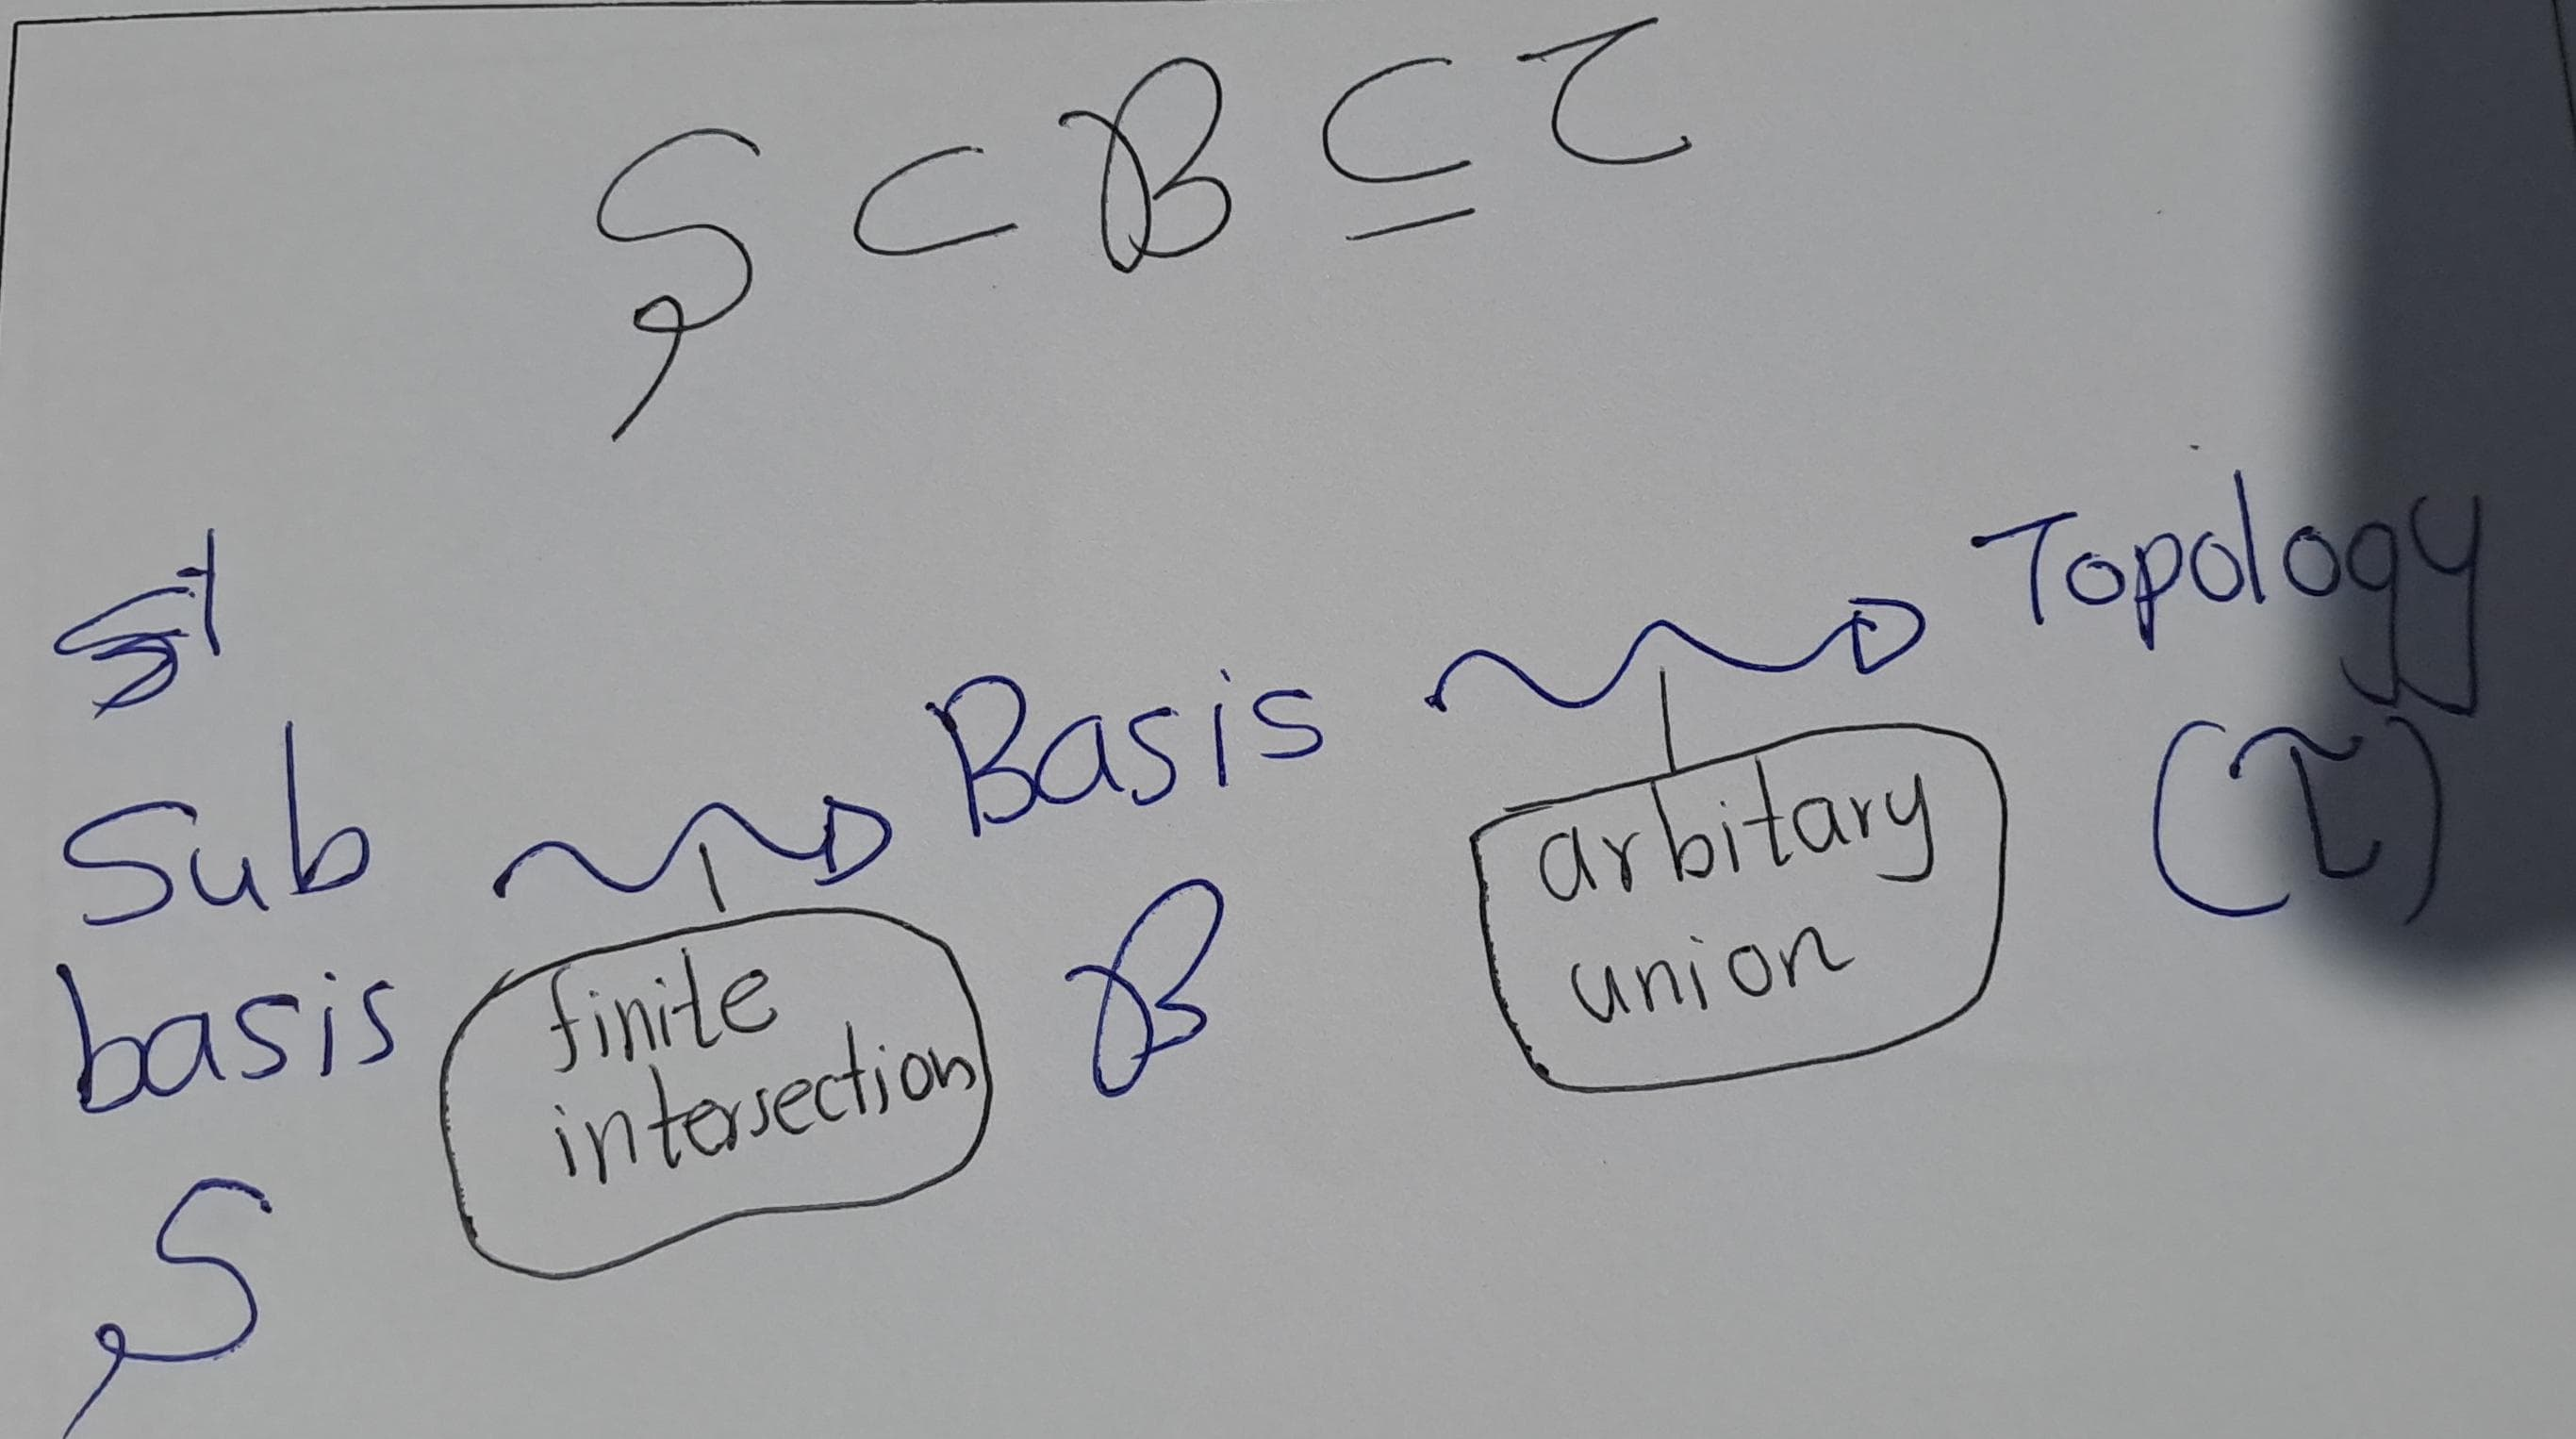
\includegraphics{figures/figure 06.jpg}
\caption{\label{fig:64}\(~\)}
\end{figure}

\begin{definition}
\protect\hypertarget{def:unnamed-chunk-19}{}\label{def:unnamed-chunk-19}The topology generated by the subbasis \(\mathcal{S}\) is defined to be the collection \(\mathcal{T}\) of all unions of finite intersections of elements of \(\mathcal{S}\).
\end{definition}

\hypertarget{order-topology}{%
\section{Order Topology}\label{order-topology}}

\begin{definition}[Linear Order/ Complete Order]
\protect\hypertarget{def:unnamed-chunk-20}{}\label{def:unnamed-chunk-20}

Consider order relation ``\(<\)''.

\begin{enumerate}
\def\labelenumi{\arabic{enumi}.}
\tightlist
\item
  If \(x \neq y\), then either \(x < y\) or \(y < x\).
\item
  If \(x < y\), then \(x\neq y\).
\item
  If \(x < y\) and \(y < z\), then \(x < z\).
\end{enumerate}

\end{definition}

\begin{example}
\protect\hypertarget{exm:unnamed-chunk-21}{}\label{exm:unnamed-chunk-21}\(\mathbb{R}\) is ordered set with less than relation.
\end{example}

First, let's see intervals in an Ordered Set.

Suppose that \(X\) is a set having a simple order relation \(<\). Given elements \(a\) and \(b\)
of \(X\) such that \(a < b\), there are four subsets of \(X\) that are called the intervals determined by \(a\) and \(b\). They are the following :

\begin{itemize}
\tightlist
\item
  \((a, b) = \{x\in X | a < x < b\}\) (Type: open interval in \(X\)),
\item
  \((a, b] = \{x\in X | a < x ≤ b\}\)(Type: half-open interval in \(X\)),
\item
  \([a, b) = \{x\in X | a ≤ x < b\}\)(Type: half-open interval in \(X\)),
\item
  \([a, b] = \{x\in X | a ≤ x ≤ b\}\) (Type: closed interval in \(X\)),
\end{itemize}

The notation used here is familiar to you already in the case where \(X\) is the real line,but these are intervals in an arbitrary ordered set.

The use of the term ``open'' in this connection suggests that open intervals in \(X\) should turn out to be open sets when
we put a topology on \(X\). And so they will.

\begin{definition}
\protect\hypertarget{def:unnamed-chunk-22}{}\label{def:unnamed-chunk-22}Let \(X\) be a set with a simple order relation; assume \(X\) has more than one element. Let \(\mathcal{B}\) be the collection of all sets of the following types:

\begin{enumerate}
\def\labelenumi{\arabic{enumi}.}
\tightlist
\item
  All open intervals \((a, b)\) in \(X\).
\item
  All intervals of the form \([a_0, b)\), where \(a_0\) is the smallest element (if any) of \(X\).
\item
  All intervals of the form \((a, b_0]\), where \(b_0\) is the largest element (if any) of \(X\).
\end{enumerate}

i.e.:
\[\begin{aligned}
\mathcal{B}:=&\{(a,b):a<b, a,b\in X\}\\
& \bigcup \{[a,b:a<b, a_0,b\in X \text{ and if $X$ has a smallest element and $a_0$ is the smallest element}\}\\
& \bigcup \{(a,b]:a<b, a,b_0\in X \text{ and if $X$ has a largest element and $b_0$ is the largest element}\}
\end{aligned}\]
The collection \(\mathcal{B}\) is a basis for a topology on \(X\), which is called the order topology.
\end{definition}

\textbf{Notation}:
Denote an arbitrary element of \(\mathbb{R} \times \mathbb{R}\) by \(x \times y\), to avoid difficulty with notation.

\begin{definition}[Dictionary Oreder]
\protect\hypertarget{def:unnamed-chunk-23}{}\label{def:unnamed-chunk-23}Suppose that \(A\) and \(B\) are two sets with order relations \(<_{A}\) and \(<_{B}\) respectively. Define an order relation \(<\) on \(A \times B\) by defining \(a_{1} \times b_{1} < a_{2} \times b_{2}\) if \(a_{1} <_{A} a_{2}\), or if \(a_{1} = a_{2}\) and \(b_{1} <_{B} b_{2}\). It is called the dictionary order relation on \(A \times B\).
\end{definition}

\begin{example}
\protect\hypertarget{exm:unnamed-chunk-24}{}\label{exm:unnamed-chunk-24}Consider the set \(\mathbb{R} \times \mathbb{R}\) in the dictionary order. The set \(\mathbb{R} \times \mathbb{R}\) has neither a largest nor a smallest element, so the order topology on \(\mathbb{R} \times \mathbb{R}\) has as basis the collection of all open intervals of the form \((a \times b, c \times d)\) for \(a < c\), and for \(a = c\) and \(b < d\).

These two types of intervals are indicated in Figure 14.1. The sub collection consisting of only intervals of the second type is also a basis for the order topology on \(\mathbb{R} \times \mathbb{R}\), as you can check.
\end{example}

\begin{figure}
\centering
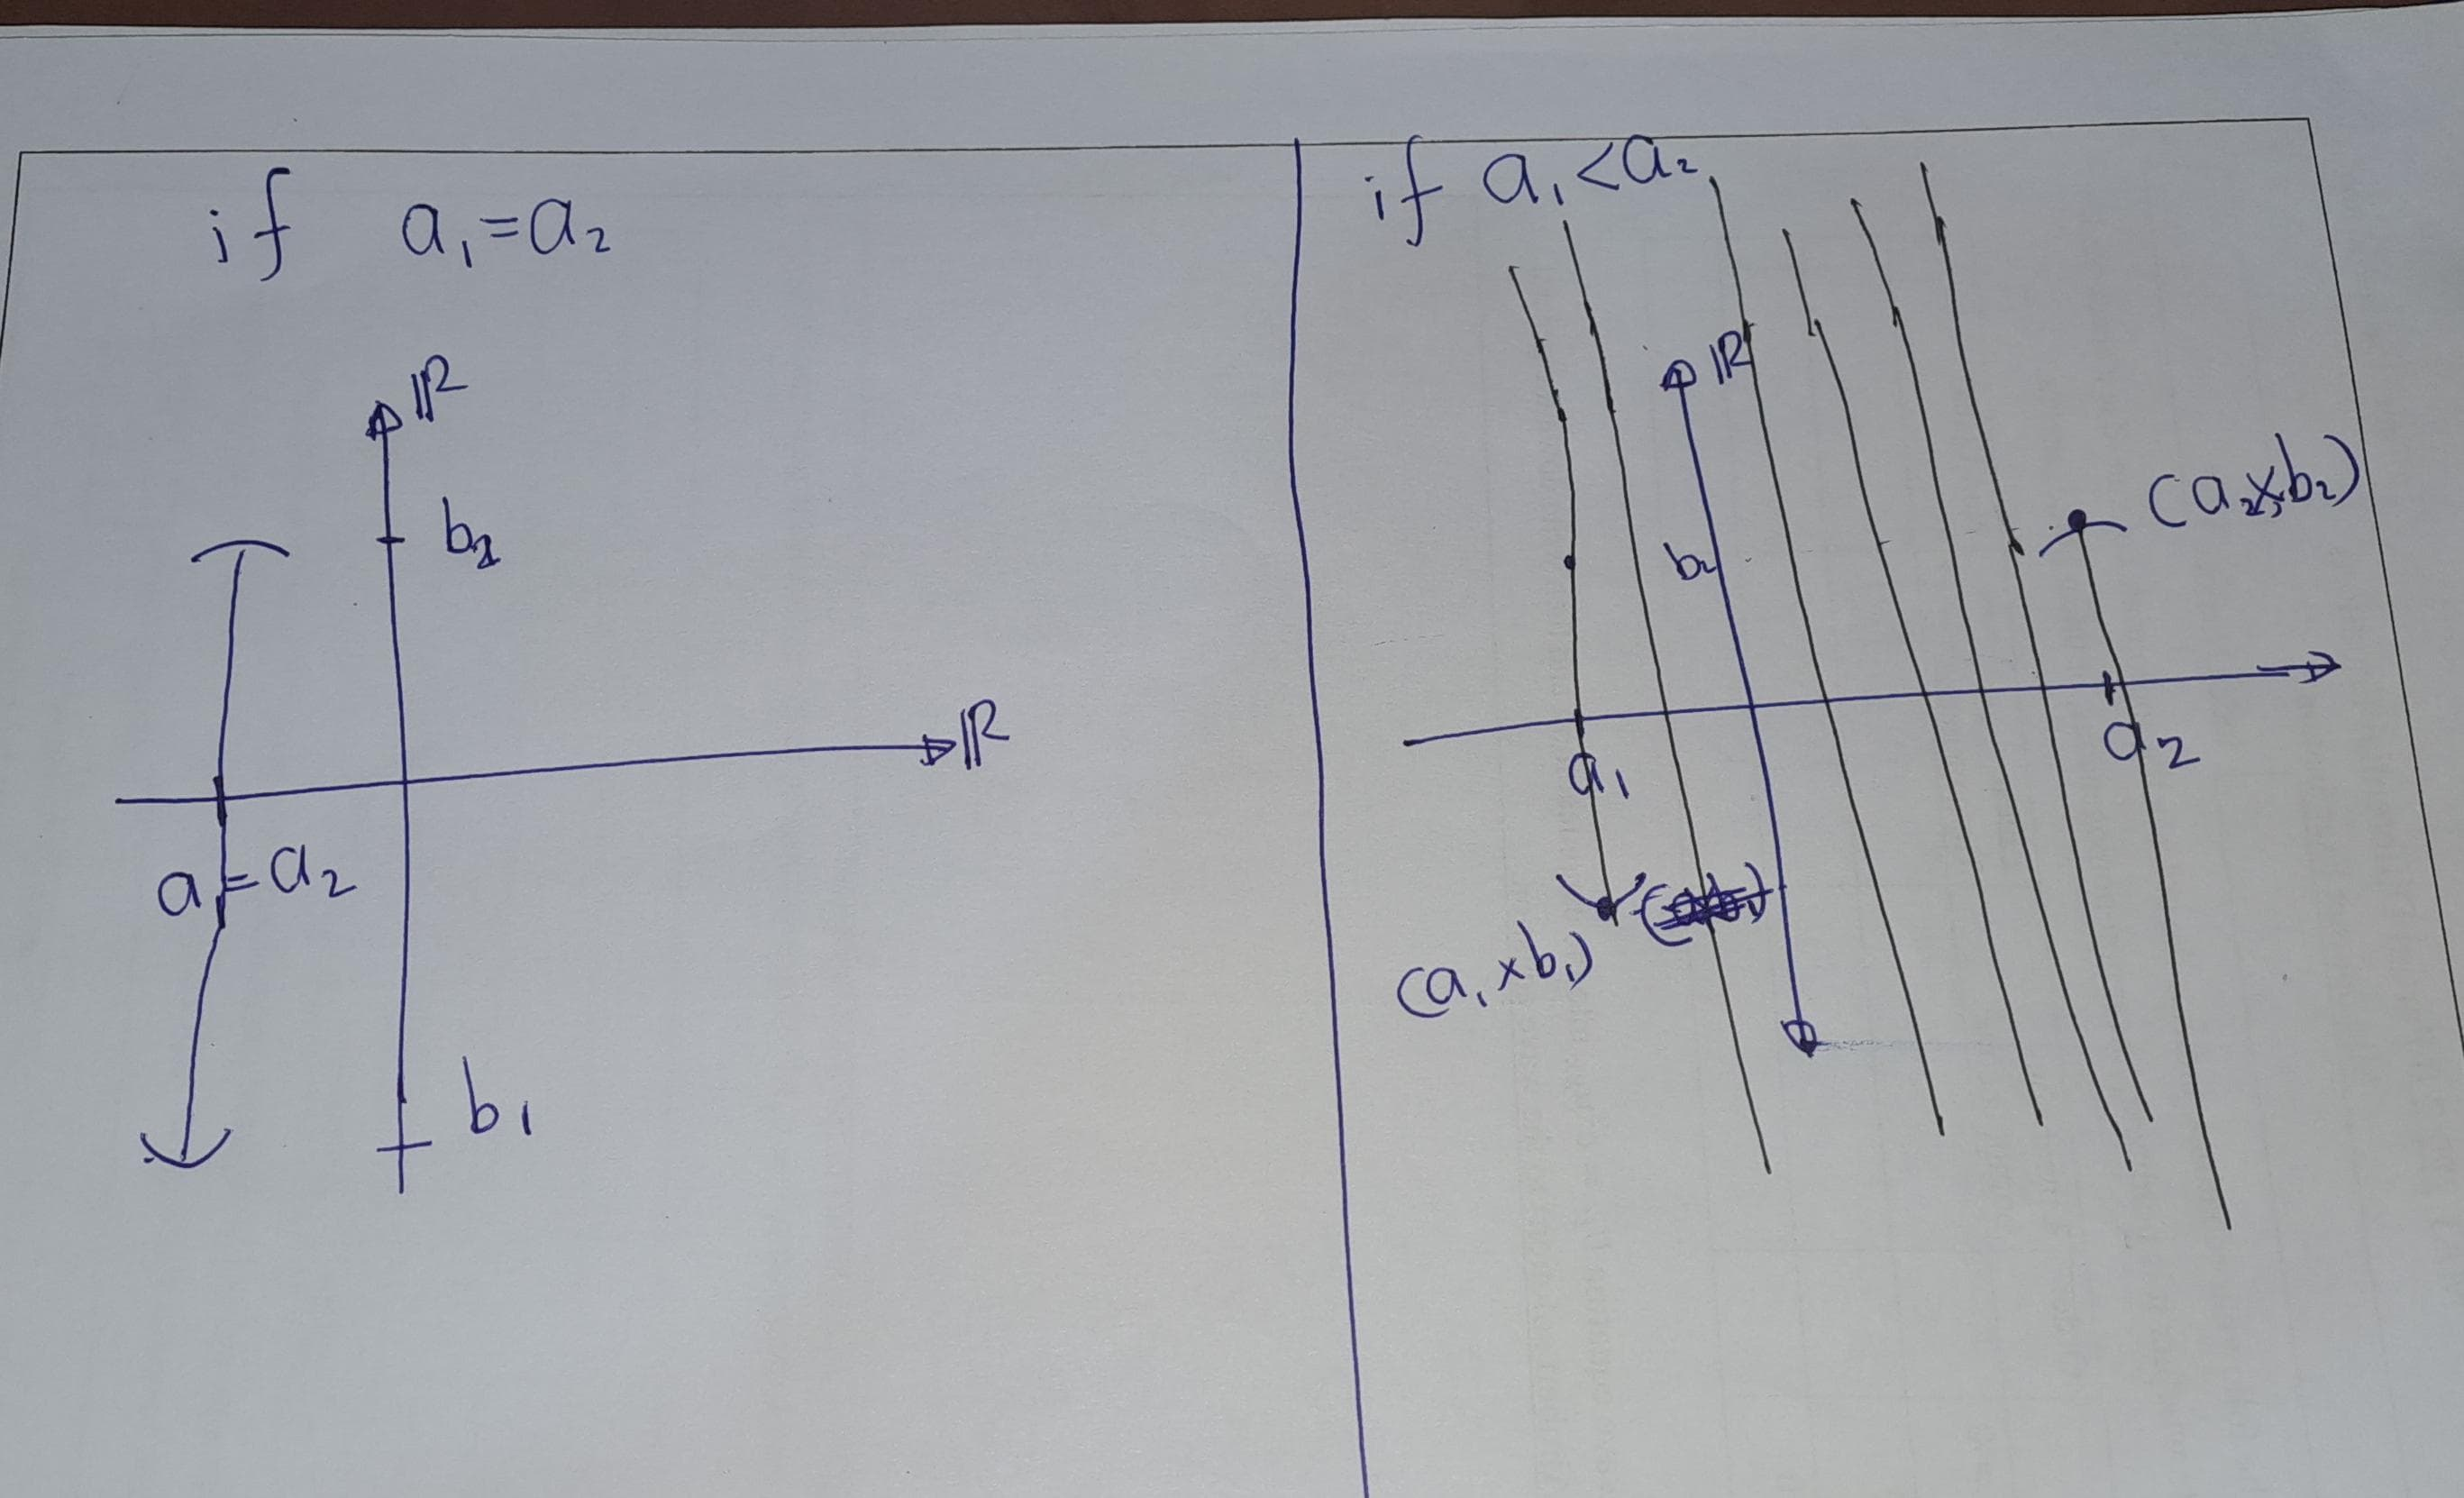
\includegraphics{figures/figure 07.jpg}
\caption{\label{fig:fi7}\(~\)}
\end{figure}

\begin{example}
\protect\hypertarget{exm:unnamed-chunk-25}{}\label{exm:unnamed-chunk-25}The standard topology,lower limit topology and upper limit topology on \(\mathbb{R}\).

\[\mathcal{B}:=\{(x,y):x<y, x,y\in \mathbb{R}\}\]
\(\mathcal{B}\) is a basis which generates the standard topology.
\[\mathcal{B}^\prime:=\{[x,y):x<y, x,y\in \mathbb{R}\}\]
\(\mathcal{B}^\prime\) is a basis which generates the lower limit topology on \(\mathbb{R}\).
\[\mathcal{B}^{\prime\prime}:=\{(x,y]:x<y, x,y\in \mathbb{R}\}\]
\(\mathcal{B}^{\prime\prime}\) is a basis which generates the upper limit topology on \(\mathbb{R}\).
\end{example}

\begin{lemma}
\protect\hypertarget{lem:unnamed-chunk-26}{}\label{lem:unnamed-chunk-26}The lower limit topology on \(\mathbb{R}\) is strictly finer than standard topology on \(\mathbb{R}\).
\end{lemma}

\begin{proof}
Let \((a,b)\in \mathbb{R}\). We are going to use Lemma \ref{lem:finerLemma}. Let \((a,b)\) be a element from basis of standard topology. Let \(x\in (a,b)\). Then \(a<x<b\). Then observe that \$ x\in [x,b)\subset (a,b) $. Note that $[x,b)$ is element of basis of lower limit topology. Thus, by lemma \\ref{lem:finerLemma} the lower limit topology on $\mathbb{R}$ is finer than standard topology on $\mathbb{R}$. Now we have to prove that **strictly property**.

Now let $[c,d)$ is element of basis of lower limit topology on $\mathbb{R}$. Now observe that there is no open interval that containing $c$ and contained in $[c,d)$. By lemma \\ref{lem:finerLemma}, the lower limit topology on $\mathbb{R}$ is strictly finer than standard topology on $\mathbb{R}$.

:::
Note that basis element in lower limit toplogy is **not** open in the standard toplogy. But otherway around is very true. As an example,
\[(1,2)=\bigcup_{n\in \mathbb{N}}[1+\frac{1}{n},2).\]
Clearly left hand side is open in lower limit toplogy by T2.

::: {.corollary #unnamed-chunk-28}
The lower limit topology on $\mathbb{R}$ is not comparable upper limit topology on $\mathbb{R}$.
:::
::: {.proof}
Exercise

Hint: (try to find counter example)
:::
**Notation**:

- $\mathbb{R}_l:=\mathbb{R}$ with lower limit topology.
- $\mathbb{R}_u:=\mathbb{R}$ with upper limit topology.
- $\mathbb{R}:=\mathbb{R}$ with standard topology.

::: {.example #unnamed-chunk-30}
The positive integers $\mathbb{Z}^+:=\{1,2,3,...\}$ form an ordered set with a smallest element. The order topology on $\mathbb{Z}^+$ is the discrete topology, for every one-point set is open: If $n > 1$, then the one-point set $\{n\} = (n - 1, n + 1)$ is a basis element; and if $n = 1$, the one-point set $\{1\}=[1, 2)$ is a basis element.
:::

![\label{fig:fig8}$~$](figures/figure 08.jpg)
::: \{.example \#unnamed-chunk-31\}
The set \(X = \{1, 2\} \times \mathbb{Z}^+\) in the dictionary order is another example of an ordered set with a smallest element. Denoting \(1 \times n\) by \(a_n\) and \(2 \times n\) by \(b_n\), we can represent \(X\) by
\[a_1, a_2,..., b_1, b_2,....\]

i.e.:\[X=\{1\times 1,1 \times 2, 1 \times 3, ..., 2\times 1, 2 \times 2, ....\}\]
Here \(a_1=1\times 1\) is the smallest element in \(X\).

The order topology on \(X\) is \textbf{not} the discrete topology. Most one-point sets are open, but there is an exception-the one-point set \(\{b_1\}={2\times 1}\). Any open set containing \(b_1\) must contain a basis element about \(b_1\) (G1 condition), and any basis element containing \(b_1\) contains points of the \(a_i\) sequence.
As an example, \(b_1=2\times 1\in (1\times 7,2\times 8)\). Then the sequence \(a_8,a_9,a_{10},....=1\times 8,1\times 9, 1\times 10,...\) contained in \((a_7,b_8)=(1\times 7,2\times 8)\). So, we cannot find an open interval in \(X\) that contains \(b_1\) and is contained in \(\{b_1\}\).
\end{proof}

\begin{example}
\protect\hypertarget{exm:unnamed-chunk-32}{}\label{exm:unnamed-chunk-32}\[\mathcal{B}^{\prime\prime\prime}:=\{[x,y]:x\leq y, x,y\in \mathbb{R}\}\]
\(\mathcal{B}^{\prime\prime\prime}\) is a basis which generates the discrete topology on \(\mathbb{R}\). Because, \(\{a\}=[a,a]\).
\end{example}

\hypertarget{product-toplogy-on-x-times-y.}{%
\section{\texorpdfstring{Product Toplogy on \(X \times Y\).}{Product Toplogy on X \textbackslash times Y.}}\label{product-toplogy-on-x-times-y.}}

The Cartesian product of two topological spaces has an induced topology called the product topology. There is also an induced basis for it. Here is the example to keep in mind:

\begin{example}
\protect\hypertarget{exm:egR2}{}\label{exm:egR2}Recall that the standard topology of \(\mathbb{R}^{2}\) is given by the basis

\[
\mathcal{B}:=\left\{(a, b) \times(c, d) \subset \mathbb{R}^{2} \mid a<b, c<d\right\}
\]
\end{example}

\begin{proof}
(Proof of \(\mathcal{B}\) is basis.)
- (B1) Let \((x,y)\in \mathbb{R}^2\). Then observe that \(x\in(x-1,x+1)\subseteq \mathbb{R}\), and \(y\in(y-1,y+1)\subseteq \mathbb{R}\). Thus
\[(x,y)\in (x-1,x+1)\times (y-1,y+1).\]

See figure \ref{fig:fig4}.
Therefore, this satisfied the B1 condition.

\begin{itemize}
\tightlist
\item
  Now suppose that \((x,y)\in (a_1,b_1)\times(c_1,d_1)\cap (a_2,b_2)\times(c_2,d_2)\)
  Now observe
  \((x,y)\in (a_1,b_1)\times(c_1,d_1)\implies x\in(a_1,b_1)\) and \(y\in(c_1,d_1)\)
\end{itemize}

and

\((x,y)\in (a_2,b_2)\times(c_2,d_2)\implies x\in(a_2,b_2)\) and \(y\in(c_2,d_2)\)
Let \(a=\max\{a_1,a_2\},b=\min\{b_1,b_2\}, c=\max\{c_1,c_2\}\) and \(d=\min\{d_1,d_2\}\). Then observe that
\[x\in (a,b)\quad \text{and} y\in (c,d)\].
Further, \[(x,y)\in (a,b)\times (c,d)\subseteq (a_2,b_2)\times(c_2,d_2)\implies x\in(a_2,b_2)\].
See figure \ref{fig:fig5}.
This satisfies B2 condition.
\end{proof}

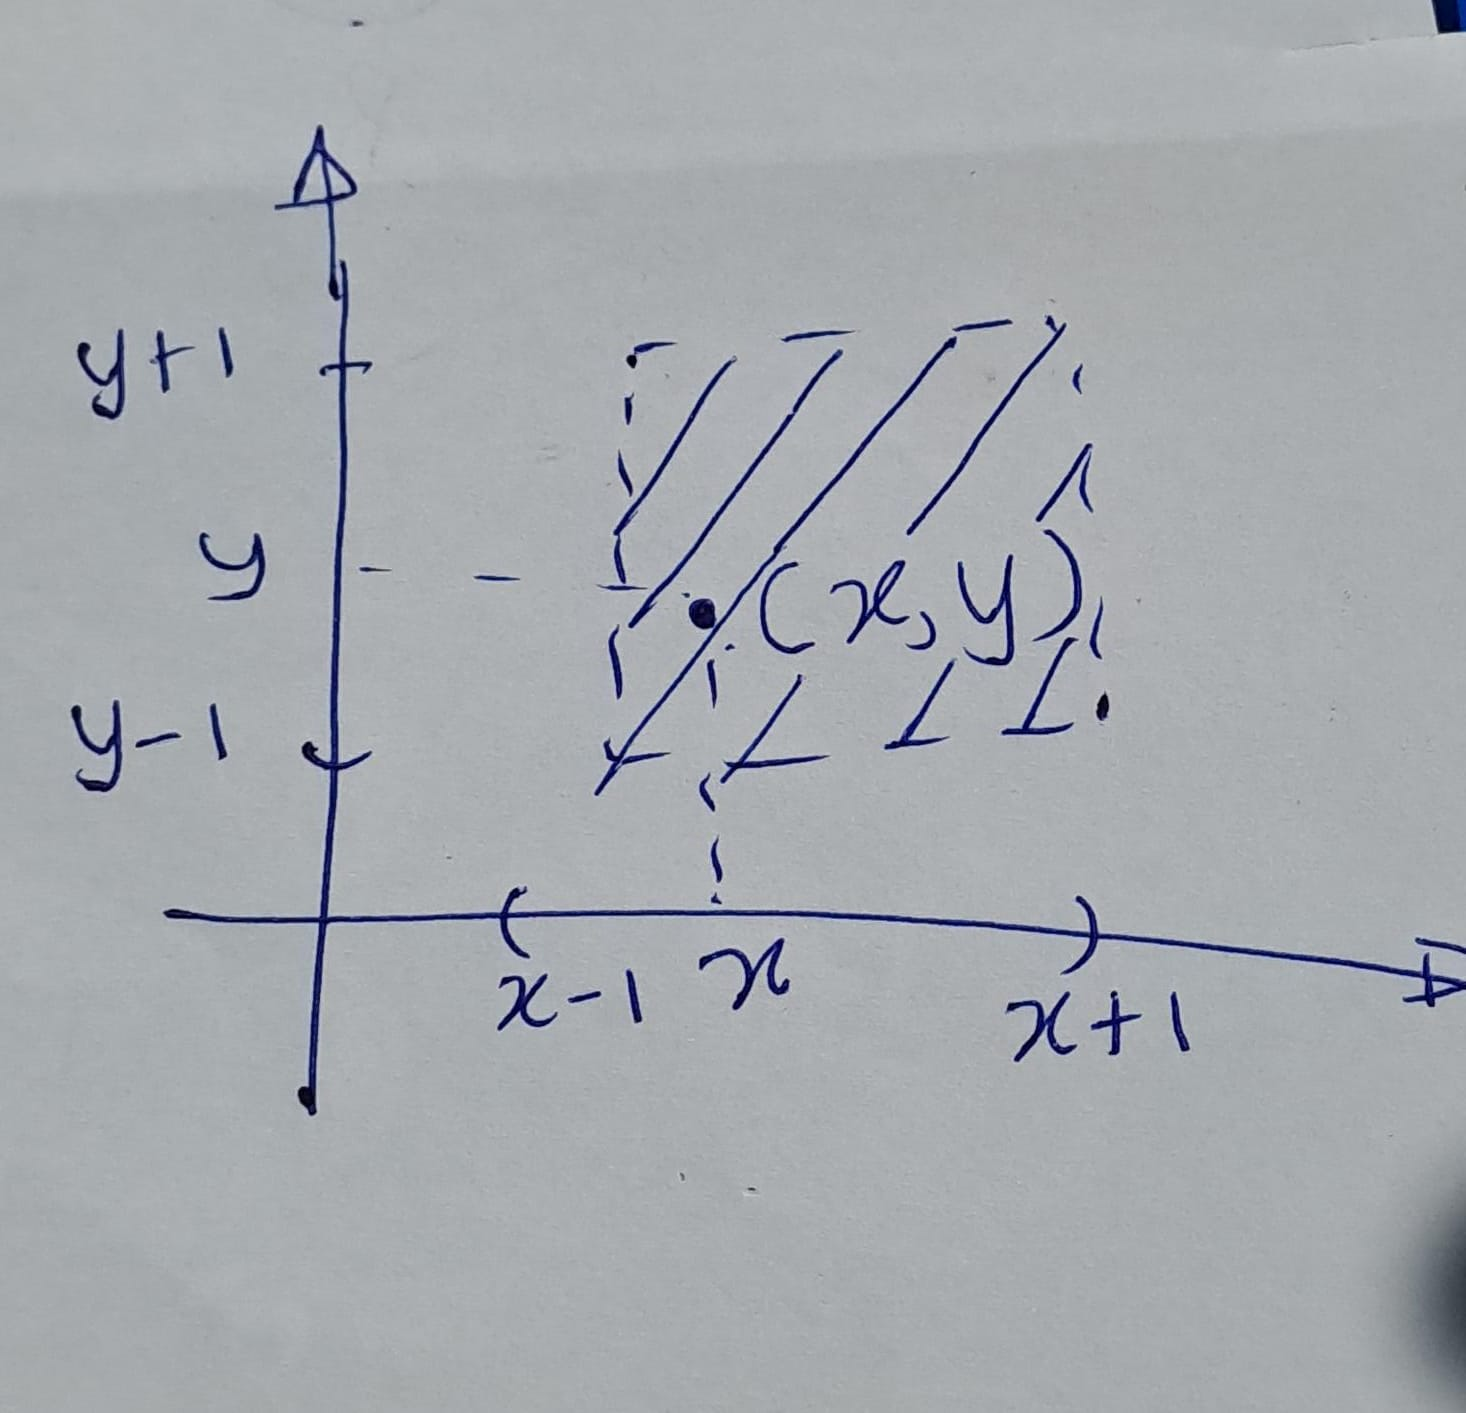
\includegraphics{figures/figure 04.jpg}
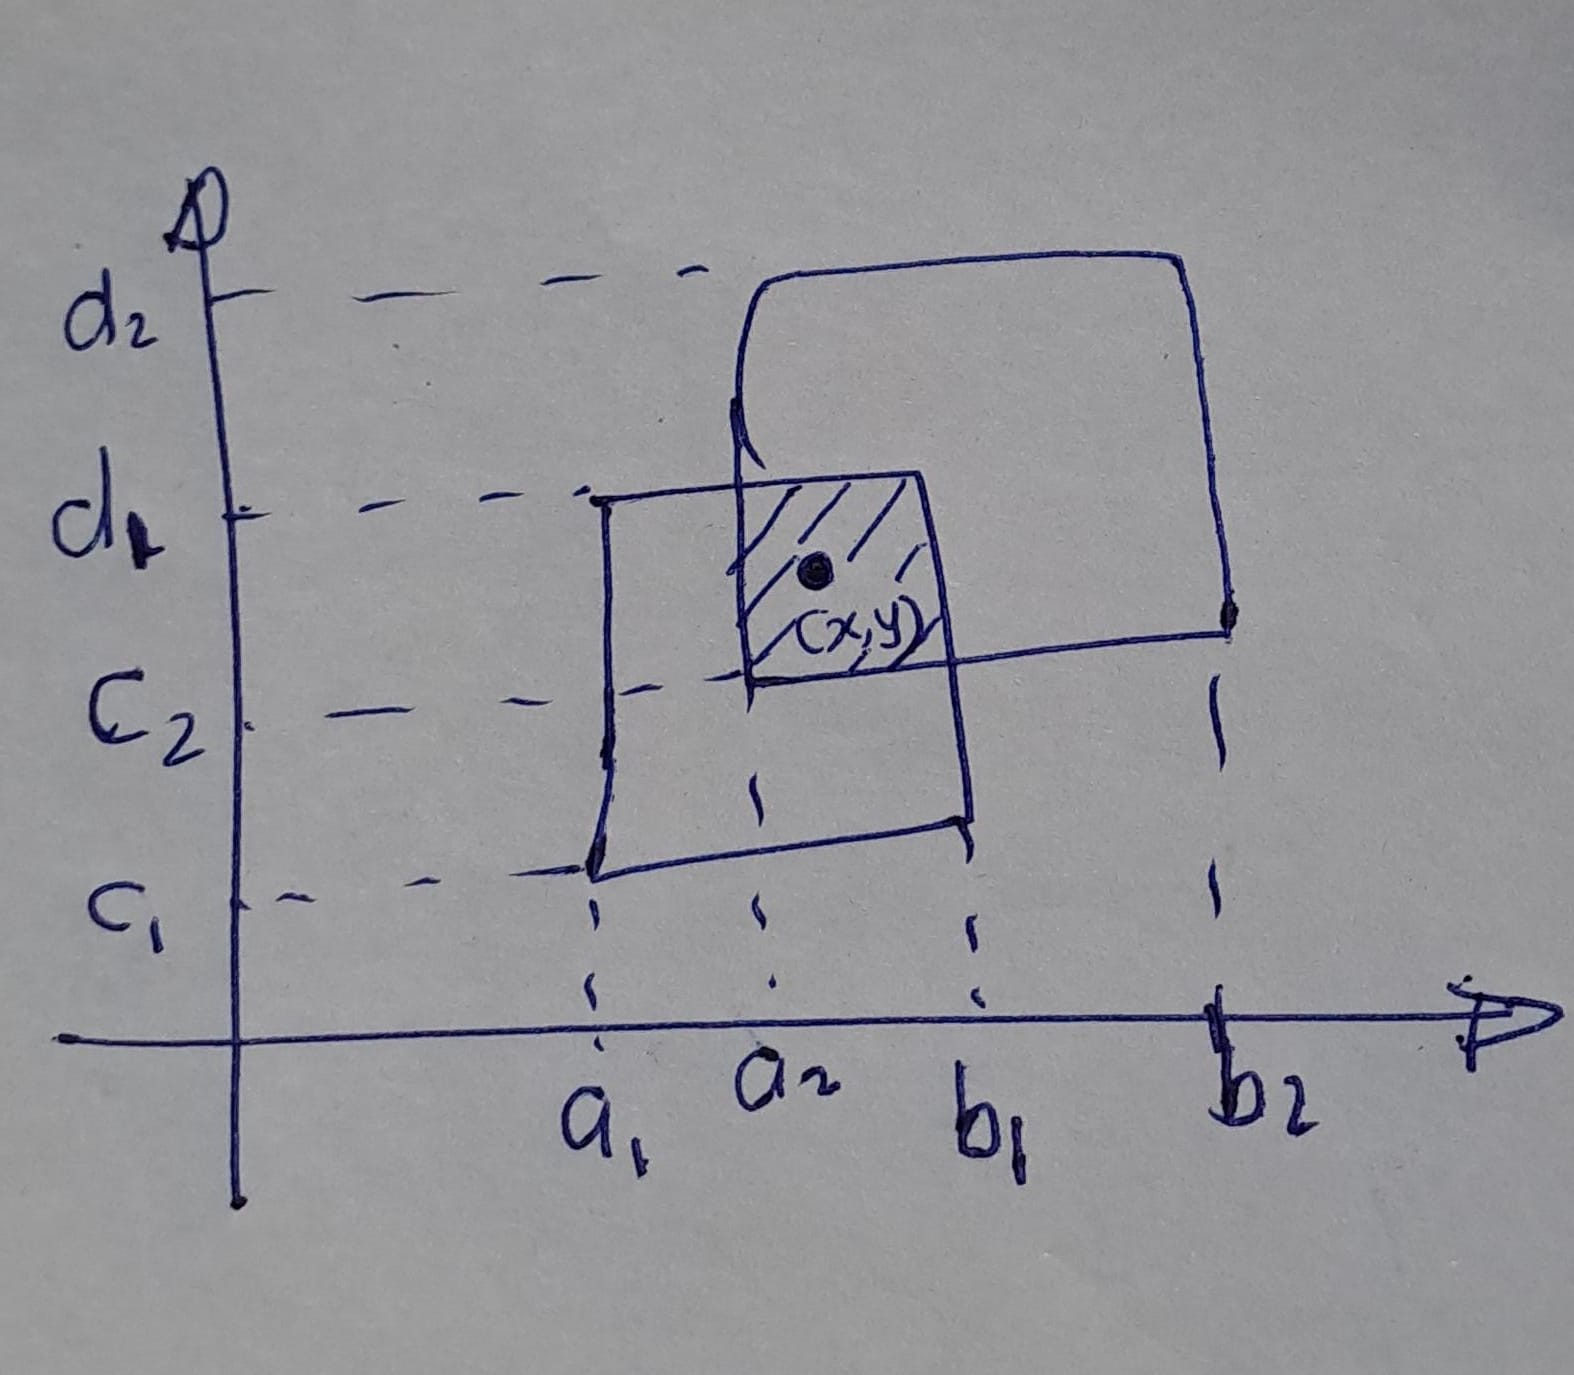
\includegraphics{figures/figure 05.jpg}
Let's go to a rigid definition.

\begin{definition}
\protect\hypertarget{def:unnamed-chunk-34}{}\label{def:unnamed-chunk-34}If \(\left(X, \mathcal{T}_{X}\right)\) and \(\left(Y, \mathcal{T}_{Y}\right)\) are topological spaces, then the collection \(\mathcal{B}\) of subsets of the form \(U \times V \subset X \times Y, U \in \mathcal{T}_{X}, V \in \mathcal{T}_{Y}\) forms a basis of a topology.

i.e.:
\[\mathcal{B}:=\{U \times V \subset X \times Y: U \in \mathcal{T}_{X}, V \in \mathcal{T}_{Y}\}\]
The topology generated by \(\mathcal{B}\) is called product topology on \(X \times Y\).
\end{definition}

\begin{proof}

(Proof of \(\mathcal{B}\) is basis)

\begin{itemize}
\item
  (B1) Let \((x, y) \in X \times Y\) be an arbitrary element. We need to find a subset in \(\mathcal{B}\) containing \((x, y)\), but since \(X \times Y \in \mathcal{B}\), it is obvious.
\item
  (B2) For any \(U_{1} \times V_{1}, U_{2} \times V_{2} \in \mathcal{B}\), the intersection is \(\left(U_{1} \times V_{1}\right) \cap\left(U_{2} \times V_{2}\right)=\left(U_{1} \cap U_{2}\right) \times\left(V_{1} \cap V_{2}\right) \in \mathcal{B}\). So it is obvious again.
\end{itemize}

\end{proof}

\begin{figure}
\centering
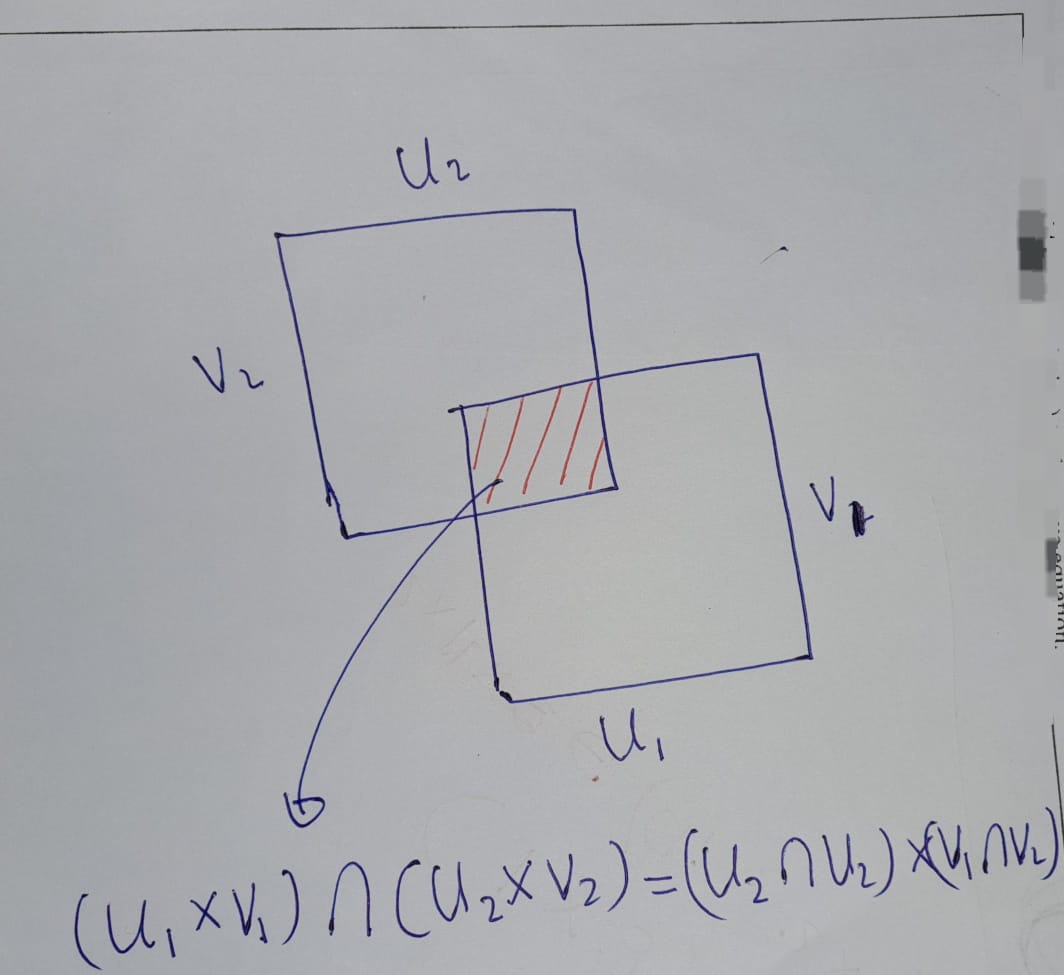
\includegraphics{figures/figure 09.jpg}
\caption{\label{fig:fig09}\(~\)}
\end{figure}

\begin{theorem}
\protect\hypertarget{thm:unnamed-chunk-36}{}\label{thm:unnamed-chunk-36}If \(\mathcal{B}_X\) is a basis of \((X, \mathcal{T}_X)\) and \(\mathcal{B}_Y\) is a basis of \((Y, \mathcal{T}_Y)\), then \(\mathcal{B}_X \times \mathcal{B}_Y\) is a basis of the product topology on \(X \times Y\).
\end{theorem}

\begin{proof}
To check \(\mathcal{B}_{X \times Y}\), let's use lemma \ref{lem:lemma110} which states that \(\mathcal{B}\) is a basis for \(\mathcal{T}\) iff for any \(U \in T\) and any \(x \in U\), there is \(B \in \mathcal{B}\) such that \(x \in B \subseteq U\).

Let \(W \in \mathcal{T}_{prod}\) and \((x, y) \in W\). By the definition of product topology, there are \(U \in \mathcal{T}_X\) and \(V \in \mathcal{T}_Y\) such that \((x,y) \in U \times V \subseteq W\). Since \(\mathcal{B}_X\) and \(\mathcal{B}_Y\) are bases, there are \(B \in \mathcal{B}_X\) and \(C \in \mathcal{B}_Y\) such that \(x \in B \subseteq U\) and \(y \in C \subseteq V\). Thus we found \(B \times C \in \mathcal{B}_{X \times Y}\) such that \((x,y) \in B \times C \subseteq W\).
\end{proof}

\begin{example}
\protect\hypertarget{exm:unnamed-chunk-38}{}\label{exm:unnamed-chunk-38}The standard topology on \(\mathbb{R}^2=\mathbb{R}\times\mathbb{R}\) is the product toplogy. (See example \ref{exm:egR2})

Obsereve that basis elements in product topology in \(\mathbb{R}^2\) are open recatngles (product of two open intervals.).
\end{example}

\begin{figure}
\centering
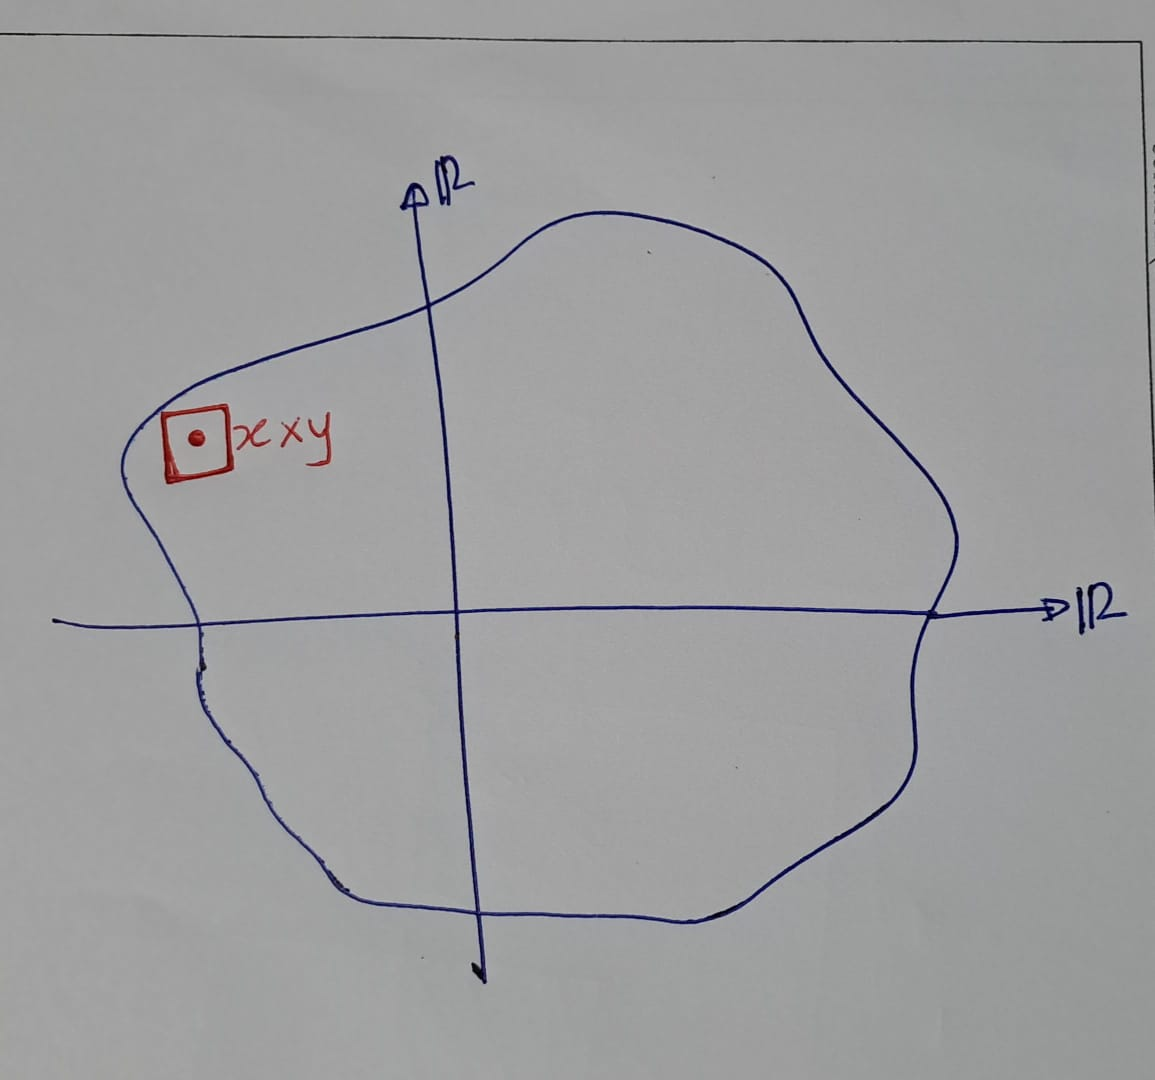
\includegraphics{figures/figure 10.jpg}
\caption{\label{fig:fig10}\(~\)}
\end{figure}

\begin{lemma}
\protect\hypertarget{lem:unnamed-chunk-39}{}\label{lem:unnamed-chunk-39}The dictionary topology \(\mathbb{R}^2\) is strictly finer than standard toplogy in \(\mathbb{R}^2\)
\end{lemma}

\begin{proof}
We are going to use \ref{lem:finerLemma}.
Let \((a,b)\times(c,d)\subset\mathbb{R}^2\) be a element of basis of standard toplogy on \(\mathbb{R}^2\), and let \(x\times y\in (a,b)\times (c,d)\). Now we need to find basis element of the dictionary order topology that contained in \((a,b)\times (c,d)\).
So,
\[x\times y \in (x\times c ,x\times d)\subset (a,b)\times(c,d).\]
Note that \((x\times c ,x\times d)\) is a basis element in the dictonary order topology. Now let's proove the stricly finer condition.

Let \((p\times q,p \times s)\) be basis element of order toplogy. Let \(p\times y \in (p\times q,p \times s)\). Now observe that there is no open rectangle that containing \(p\times y\) and contained in \((p\times q,p \times s)\). By lemma \ref{lem:finerLemma}, the order topology on \(\mathbb{R}^2\) is strictly finer than standard topology on \(\mathbb{R}^2\).
\end{proof}

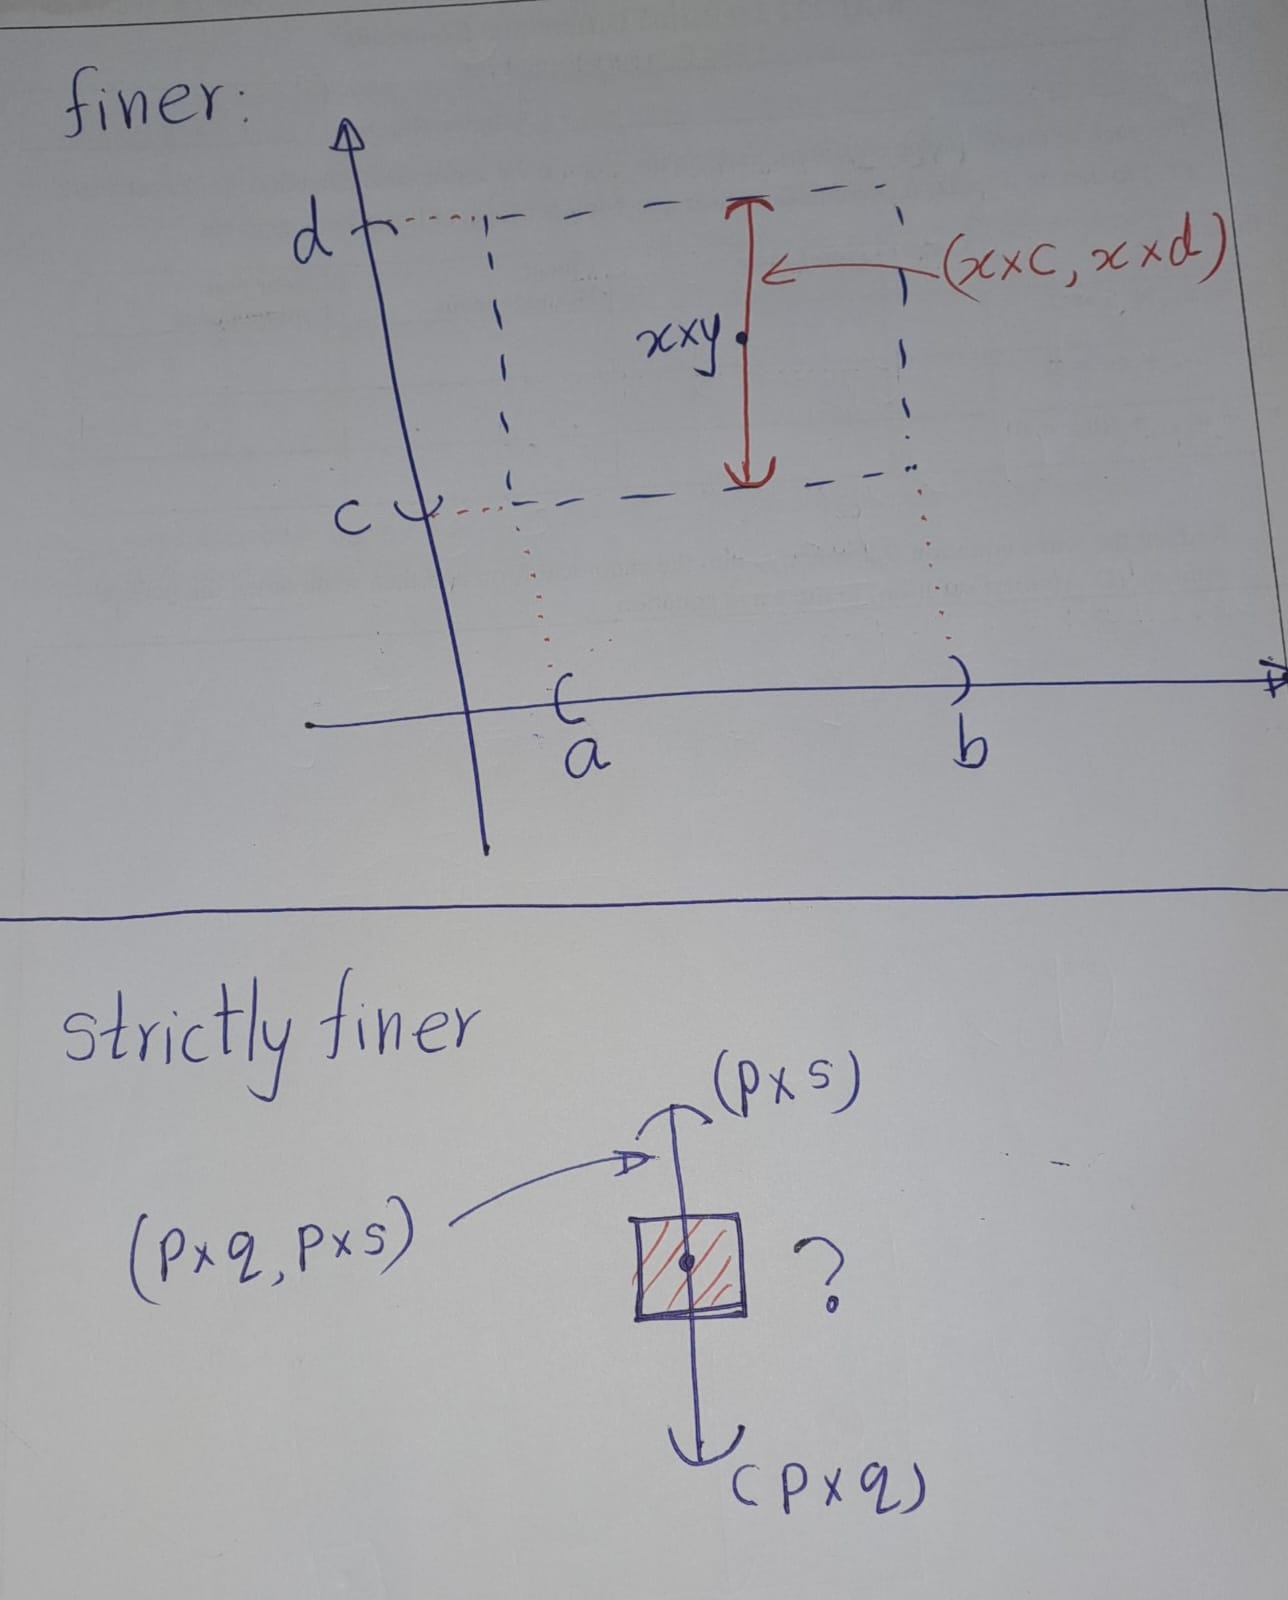
\includegraphics{figures/figure 11.jpg}
Now I am intersected in a problem. That is can we write dictionary order topology as \(\mathbb{R}^2\) as product topology. Actually we can,
\[\mathbb{R}^2_{dictionary}:=\mathbb{R}_{discrete }\times \mathbb{R}_{standard}\]

\begin{proof}
Let \(\{a\} \times (c,d)\) be a basis element in product toplogy \(\mathbb{R}_d \times \mathbb{R}\). Let \(a\times x\in \{a\} \times (c,d)\) obsereve that
\[a\times x\in \{a\} \times (c,d) = (a\times c,a\times d)\]
and \((a\times c,a\times d)\) is basis element of order topology \(\mathbb{R}^2\). Thus by lemma \ref{lem:finerLemma}, order toplogy in \(\mathbb{R}^2\) is finer than the product toplogy \(\mathbb{R}_d \times \mathbb{R}\).

Now suppose that \((p\times q, r \times s)\) be a basis elemenet in order toplogy on \(\mathbb{R}^2\).

\begin{itemize}
\tightlist
\item
  If \(p<x\), define \(l=y−1\) and if \(p=x\) define \(l=r\). In either case we know that \((p\times q)<(x\times l)<(x\times y)\).
\item
  If \(x<r\) define \(t=y+1\) and if \(x=r\) define \(t=s\). In either case we know that \((x\times y)<(x\times t)<(q \times s)\).
\end{itemize}

See figure \ref{fig:fig12}
So \[(x,y) \in \{x\} \times (l,t) \subseteq (p \times q, r \times s).\]
Thus by lemma \ref{lem:finerLemma}, product toplogy \(\mathbb{R}_d \times \mathbb{R}\) is finer than order toplogy in \(\mathbb{R}^2\).

Therefore, \[\mathbb{R}^2_{dictionary}=\mathbb{R}_{discrete }\times \mathbb{R}_{standard}\]
\end{proof}

\begin{figure}
\centering
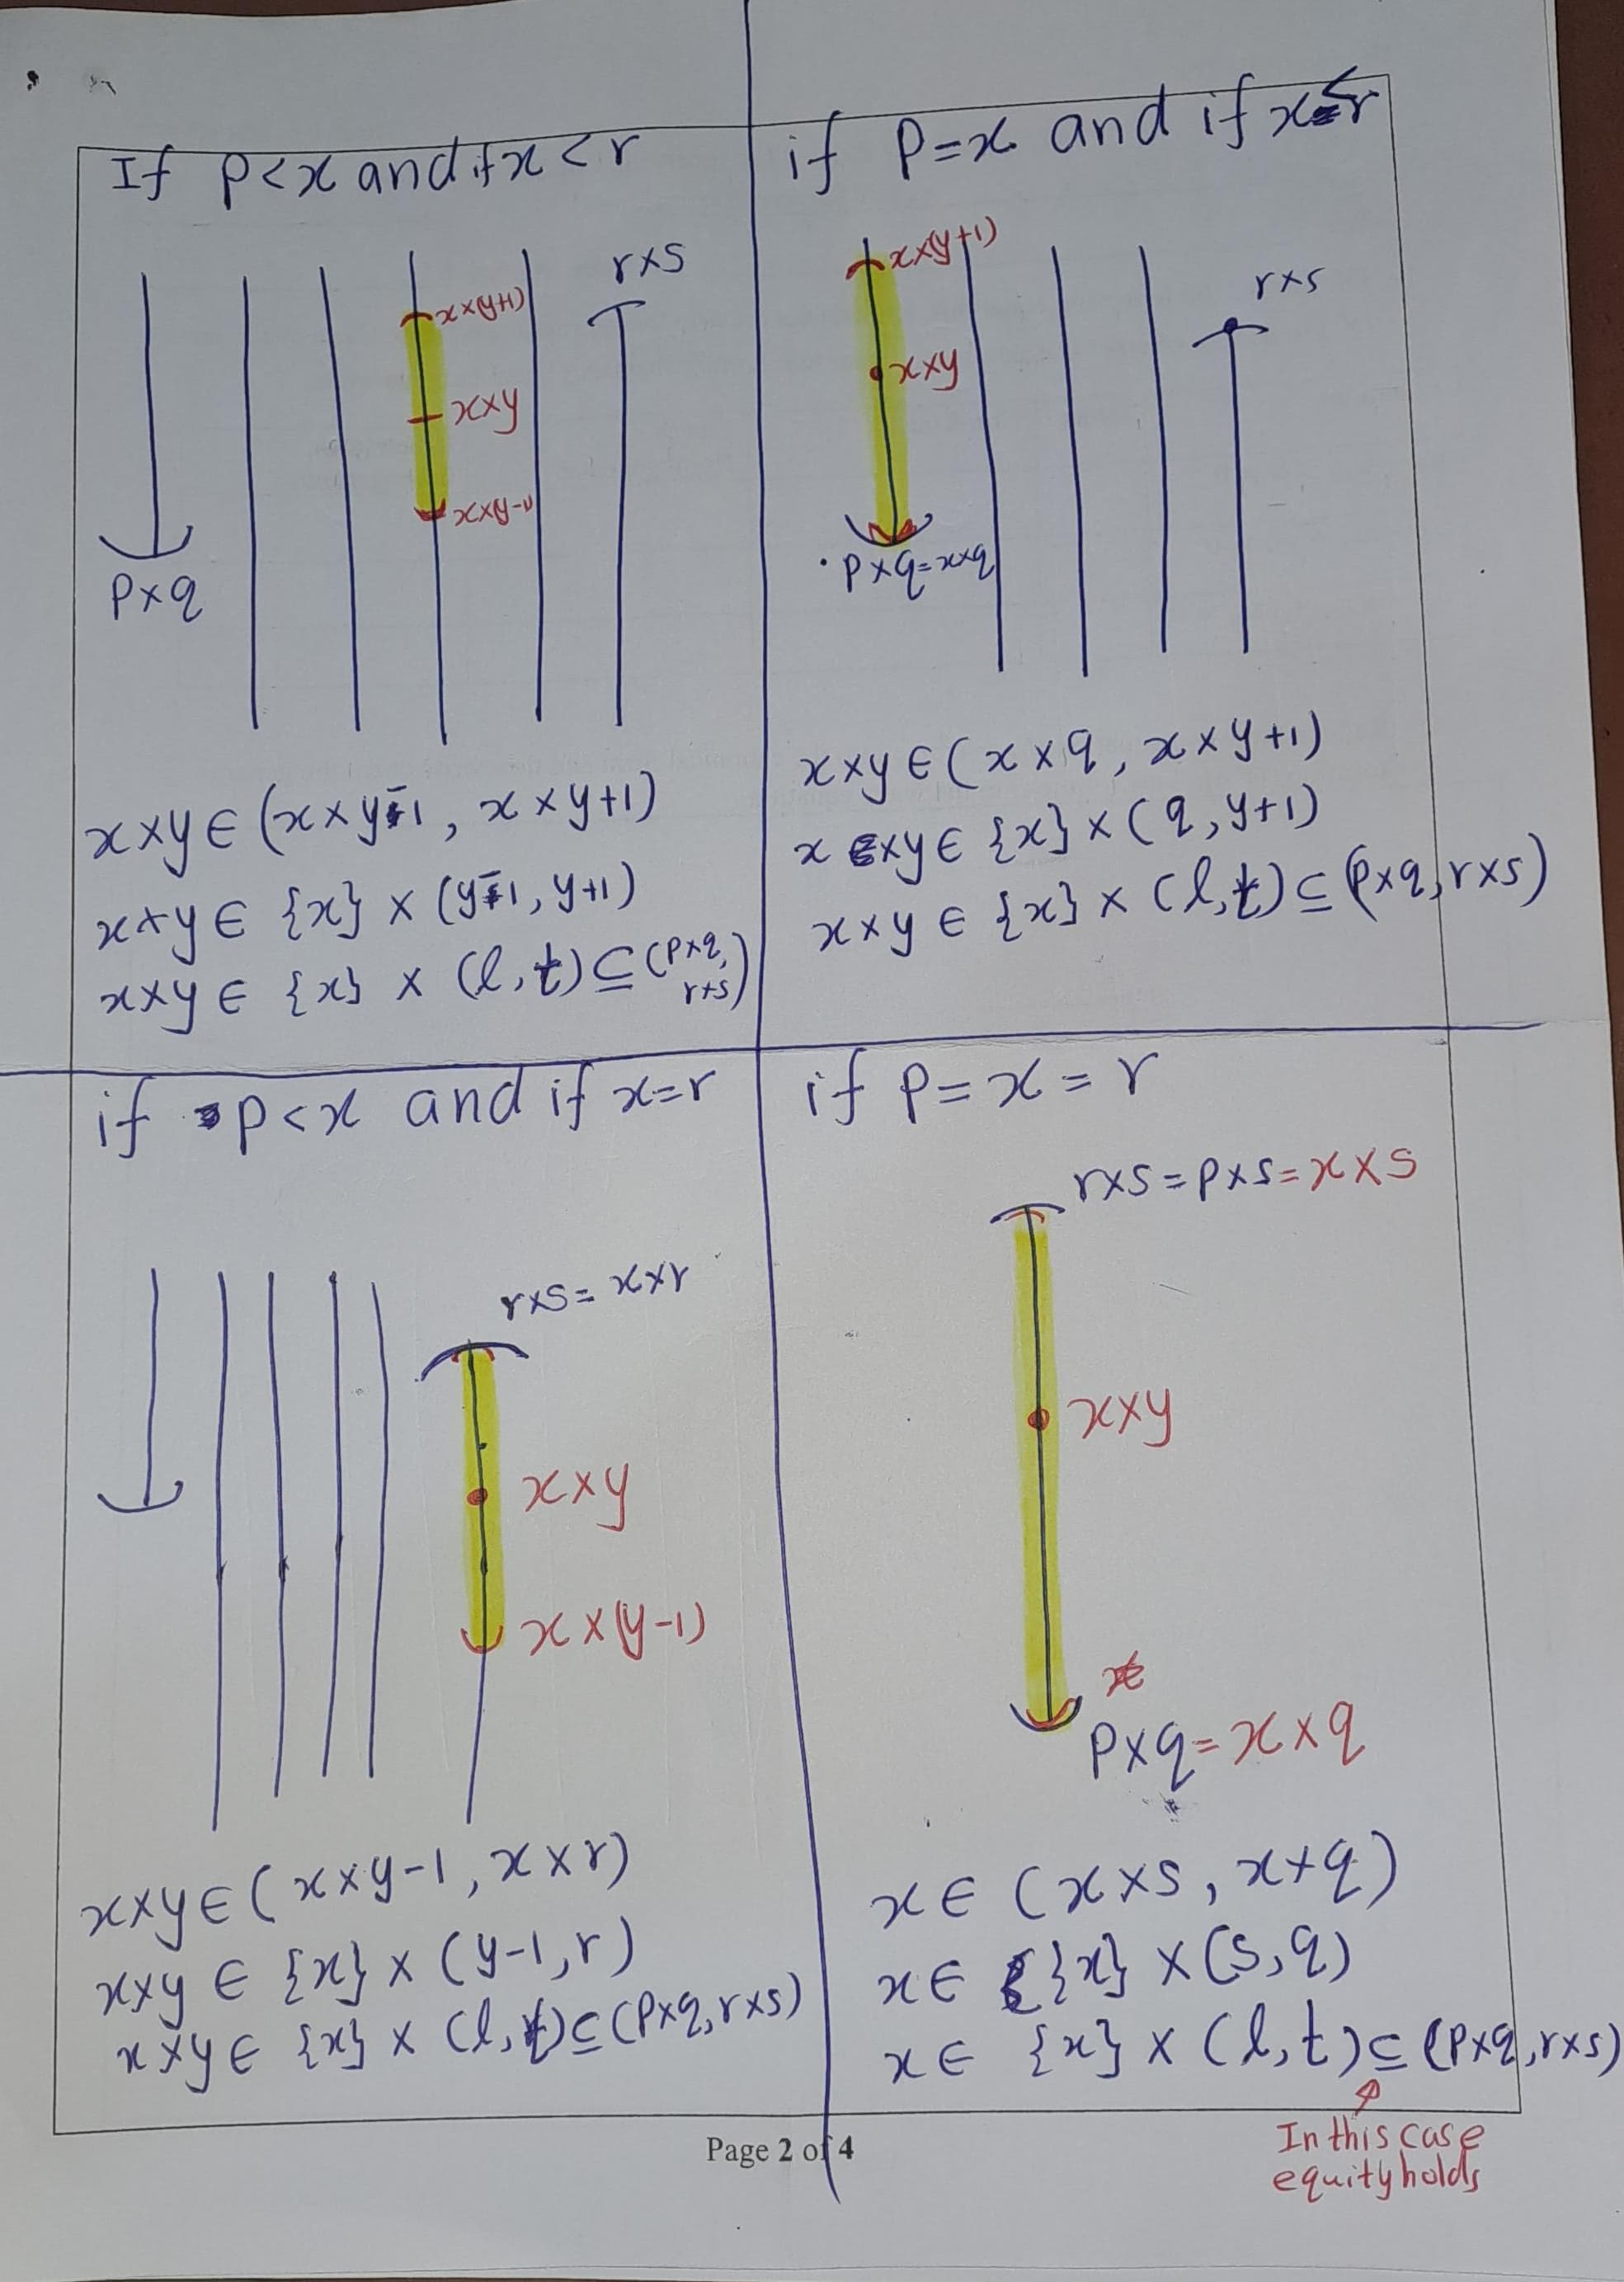
\includegraphics{figures/figure 12.jpg}
\caption{\label{fig:fig12}\(~\)}
\end{figure}

\hypertarget{the-subspace-topology}{%
\section{The Subspace Topology}\label{the-subspace-topology}}

\emph{A subset of a topological space has a naturally induced topology, called the subspace topology. In geometry, the subspace topology is the source of all funky typologies.}

\begin{definition}
\protect\hypertarget{def:unnamed-chunk-42}{}\label{def:unnamed-chunk-42}Let \((X, \mathcal{T})\) be a topological space. Let \(Y\subseteq X\). The collection
\[\mathcal{T}_Y = \{Y \cap U | U \in \mathcal{T}\}\] is a topology on \(Y\), called the subspace topology.
\end{definition}

\begin{proof}

(Proof of the collection \(\mathcal{T}_Y\) is a tology).

\begin{itemize}
\tightlist
\item
  (T1) This is very easy to see. \(\mathcal{T}_Y\) contains \(\emptyset\) and \(Y\) because \(\emptyset = Y \cap \emptyset and Y = Y \cap X\), where \(\emptyset\) and \(X\) are elements of \(\mathcal{T}\).
\item
  (T2) Let \(\{U_\alpha \cap Y\in \mathcal{T_Y}:\alpha \in I, \text{ I is index set}\}\) be collection of open sets in subspace toplogy of \(Y\), where \(U_\alpha\in \mathcal{T}\).
  \[\bigcup_{\alpha \in I}\left(U_\alpha\cap Y\right)
    =\bigcup_{\alpha \in I}\left(U_\alpha\right)\cap Y.\]
  Thus it contains in \(\mathcal{T}\). Thus \(\mathcal{T}_Y\) is closed under arbitary unions.
\item
  (T3) Let \(U_1\cap Y, U_2\cap Y,..., U_n\cap Y\) be finite collection of open sets in subspace toplogy of \(Y\) in \(X\).
  \[(U_1\cap Y)\bigcap (U_2\cap Y)\bigcap \cdots \bigcap (U_n\cap Y)=(U_1\cap U_2 \cap \cdot U_n)\bigcap Y.\]
  Thus it contains in \(\mathcal{T}\).Thus \(\mathcal{T}_Y\) is closed under finite intersections.
\end{itemize}

\end{proof}

\begin{lemma}
\protect\hypertarget{lem:unnamed-chunk-44}{}\label{lem:unnamed-chunk-44}Let \((X, \mathcal{T})\) be a topological space, and \(Y\subseteq X\). If \(\mathcal{B}\) is a basis for \(\mathcal{T}\) then the collection
\[\mathcal{B}_Y = \{B \cap Y | B \in \mathcal{B}\}\]
is a basis for the subspace topology on \(Y\).
\end{lemma}

\begin{proof}
Let \(V\in \mathcal{T}_Y\). Then \(V=U\cap Y\) for some \(U\in \mathcal{T}\). For every \(x \in V\), there is \(B \in \mathcal{B}\) such that \(x \in B \subset U\) since \(\mathcal{B}\) is a basis of \(\mathcal{T}\) (Lemma \ref{lem:lemmaTequalsTB}). Now we found \(Y \cap B\) such that \(x \in Y \cap B \subset V\).
\end{proof}

\begin{figure}
\centering
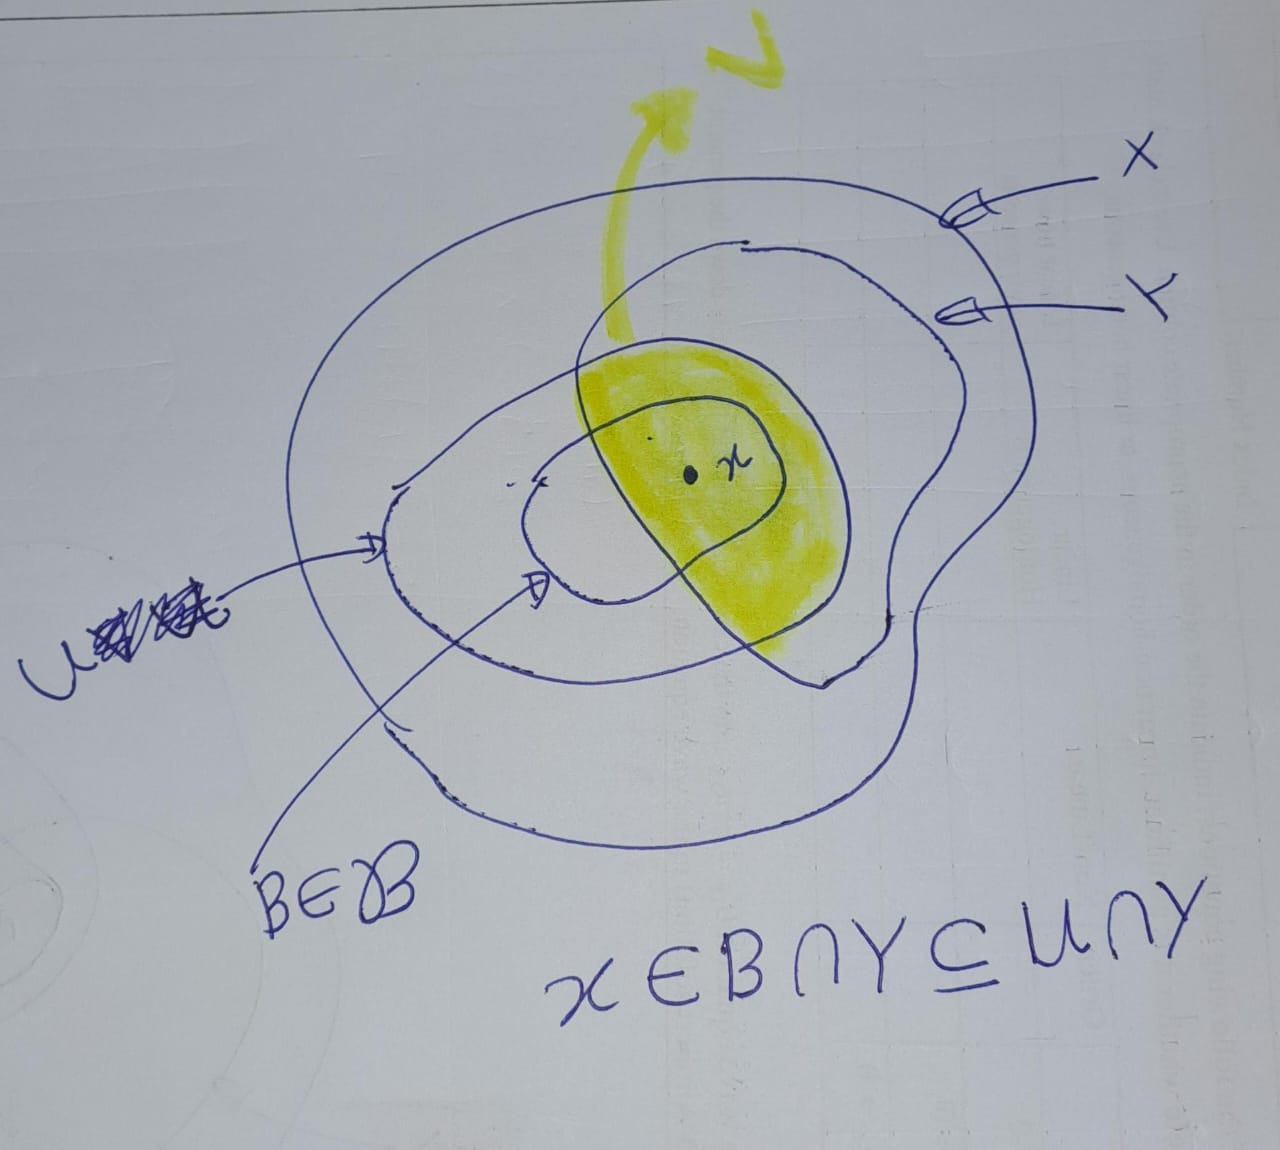
\includegraphics{figures/figure 13.jpg}
\caption{\label{fig:fig13}\(~\)}
\end{figure}

\begin{example}
\protect\hypertarget{exm:unnamed-chunk-46}{}\label{exm:unnamed-chunk-46}Let \(I = [0, 1]\). The dictionary order on \(I \times I\) is just the restriction to \(I \times I\) of the dictionary order on the plane \(\mathbb{R} \times \mathbb{R}\). However, the dictionary order topology on \(I \times I\) is \textbf{NOT} the same as the subspace topology on \(I \times I\) obtained from the dictionary order topology on \(\mathbb{R} \times \mathbb{R}\)!

For example, the set \(\{\frac{1}{2}\} \times (\frac{1}{2}, 1]\) is open in \(I \times I\) in the
subspace topology, but not in the order topology, as you can check.

See Figure \ref{fig:fig14}.
\end{example}

\begin{figure}
\centering
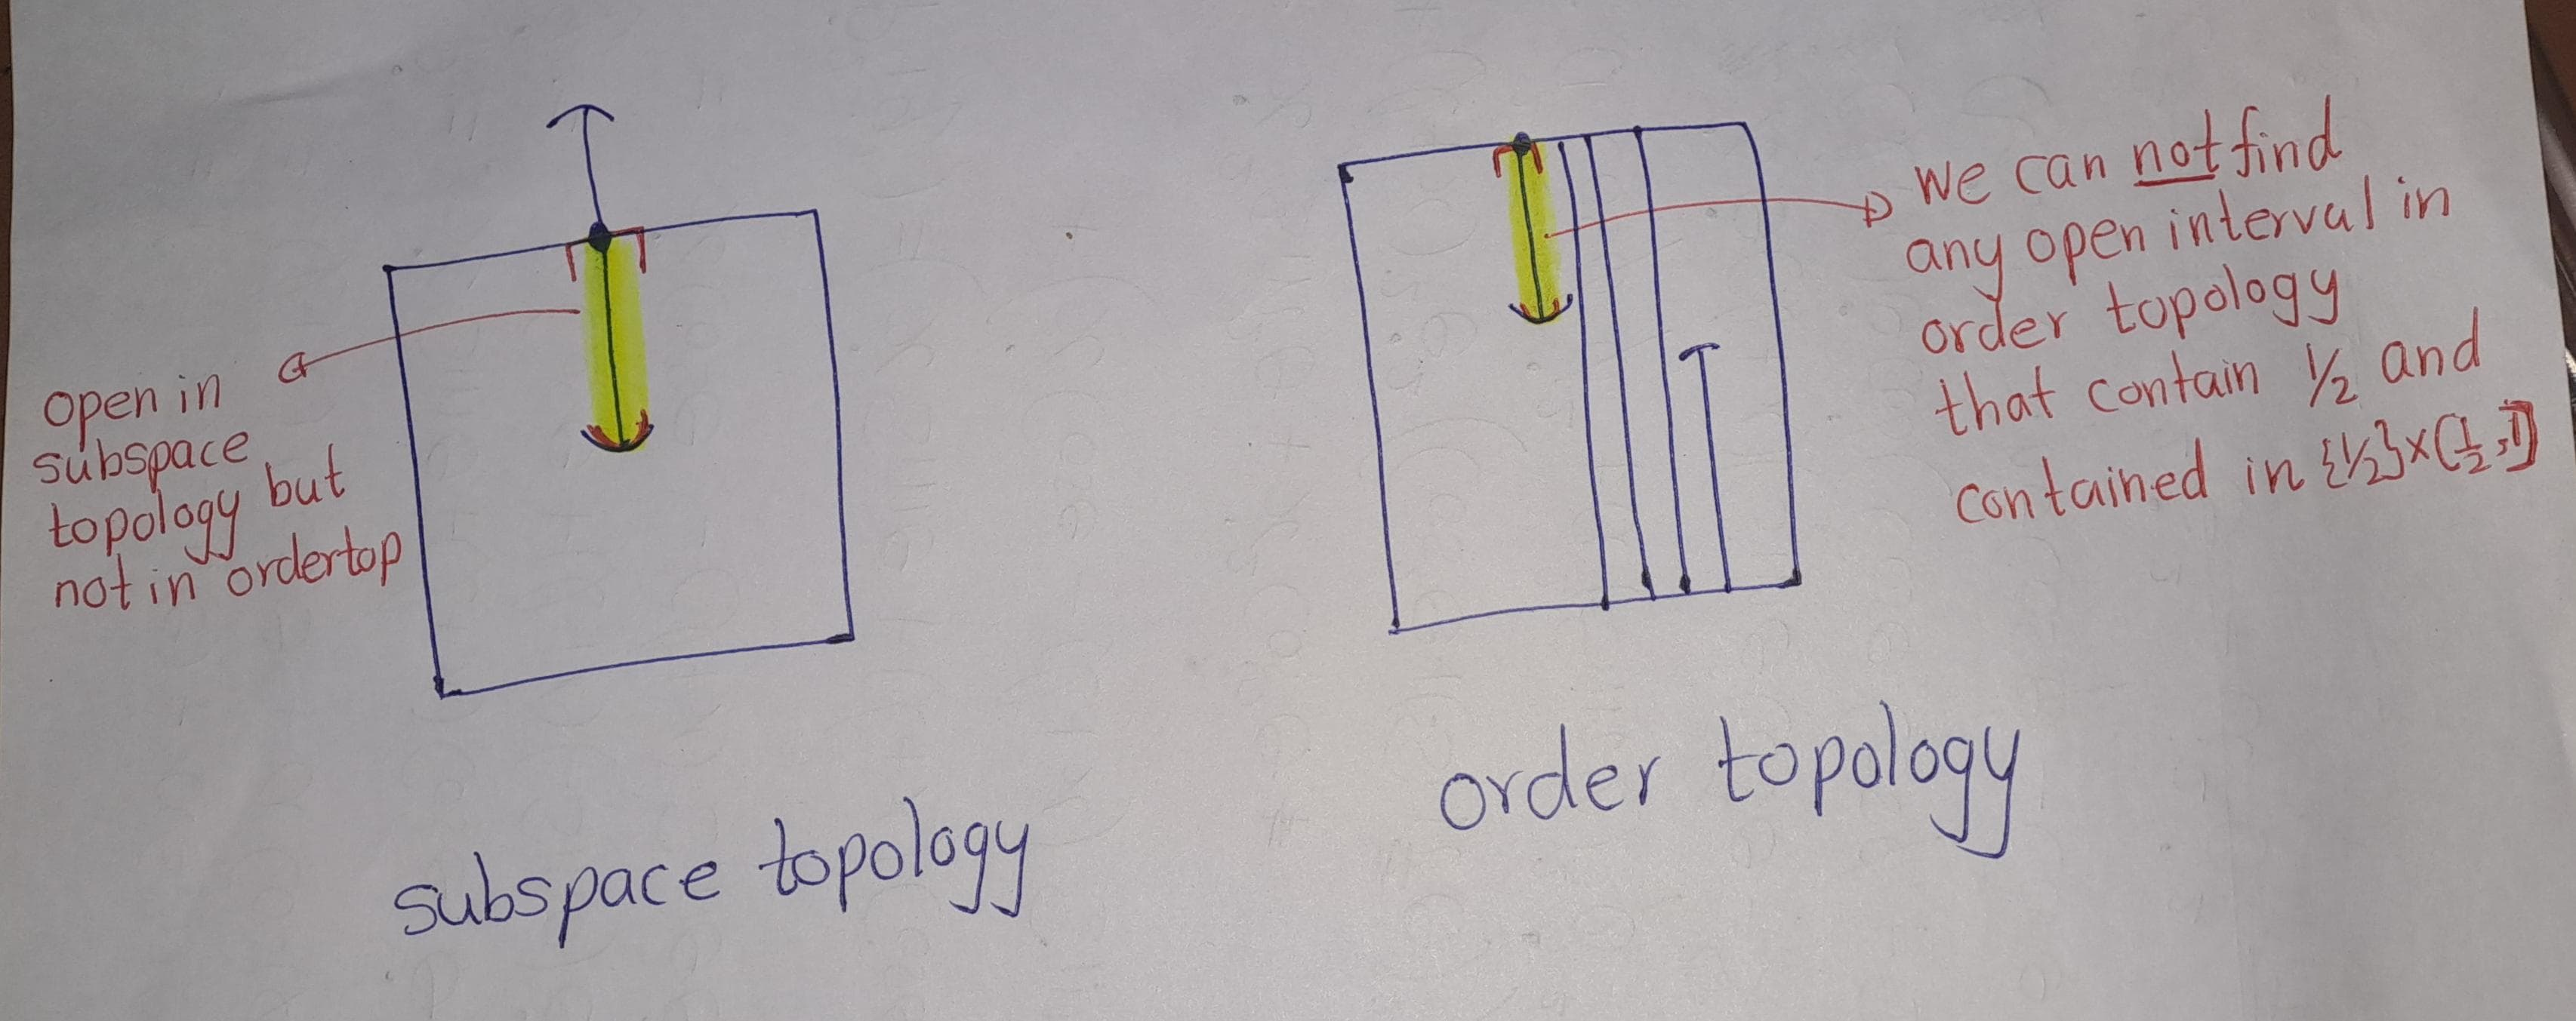
\includegraphics{figures/figure 14.jpg}
\caption{\label{fig:fig14}\(~\)}
\end{figure}

\textbf{Notation} : The set \(I \times I\) in the dictionary order topology will be called the ordered square, and
denoted by \(I_o^2\).

Let's generalized the idea.

\begin{lemma}
\protect\hypertarget{lem:unnamed-chunk-47}{}\label{lem:unnamed-chunk-47}The subspace topology on \(I \times I\) obtained from the dictionary order topology on \(\mathbb{R} \times \mathbb{R}\) is strictly finer than the dictionary order toplogy on \(I \times I\).
\end{lemma}

\begin{proof}
So, as pervious we have to proove two things they are finer condtion and strictly condition.

Let \((a_1\times b_1, a_2 \times b_2)\) be a basis elemenet of order toplogy. and \(x\times y \in (a_1\times b_1, a_2 \times b_2)\)

\begin{itemize}
\item
  \textbf{Case I} \((a_1<x<a_2)\):
  \[x\times y \in (x\times-1,x\times 2)\cap I^2= [x\times 0,x\times 1]=\{x\}\times [0,1] \subset (a_1\times b_1, a_2 \times b_2)\]
  Note that \((x\times -1,x\times 2)\cap I^2\) is a basis element of subspace topology.
\item
  \textbf{Case II} \((a_1=x<a_2)\):
  \[x\times y \in (x\times b_1,x\times 2)\cap I^2= [x\times b_1,x\times 1]=\{x\}\times (b_1,1] \subset (a_1\times b_1, a_2 \times b_2)\]
  Note that \((x\times b_1,x\times 2)\cap I^2\) is a basis element of subspace topology.
\item
  \textbf{Case III} \((a_1<x=a_2)\):
  \[x\times y \in (x\times -1,x\times b_2)\cap I^2= [x\times 0,x\times b_2]=\{x\}\times [0,b_2) \subset (a_1\times b_1, a_2 \times b_2)\]
  Note that \((x\times -1,x\times b_2)\cap I^2\) is a basis element of subspace topology.
\item
  \textbf{Case IV} \((a_1=x=a_2)\):
  \[x\times y \in (x\times b_1,x\times b_2)\cap I^2= [x\times b_1,x\times b_2]=\{x\}\times [b_1,b_2) \subset (a_1\times b_1, a_2 \times b_2)\]
  Note that \((x\times b_1,x\times b_2)\cap I^2\) is a basis element of subspace topology.
\end{itemize}

See figure \ref{fig:fig15}

In above all four cases, we have found basis element of subspace topology that conatain \(x\times y\) and conatined in \((a_1\times b_1, a_2 \times b_2)\).
\end{proof}

\begin{figure}
\centering
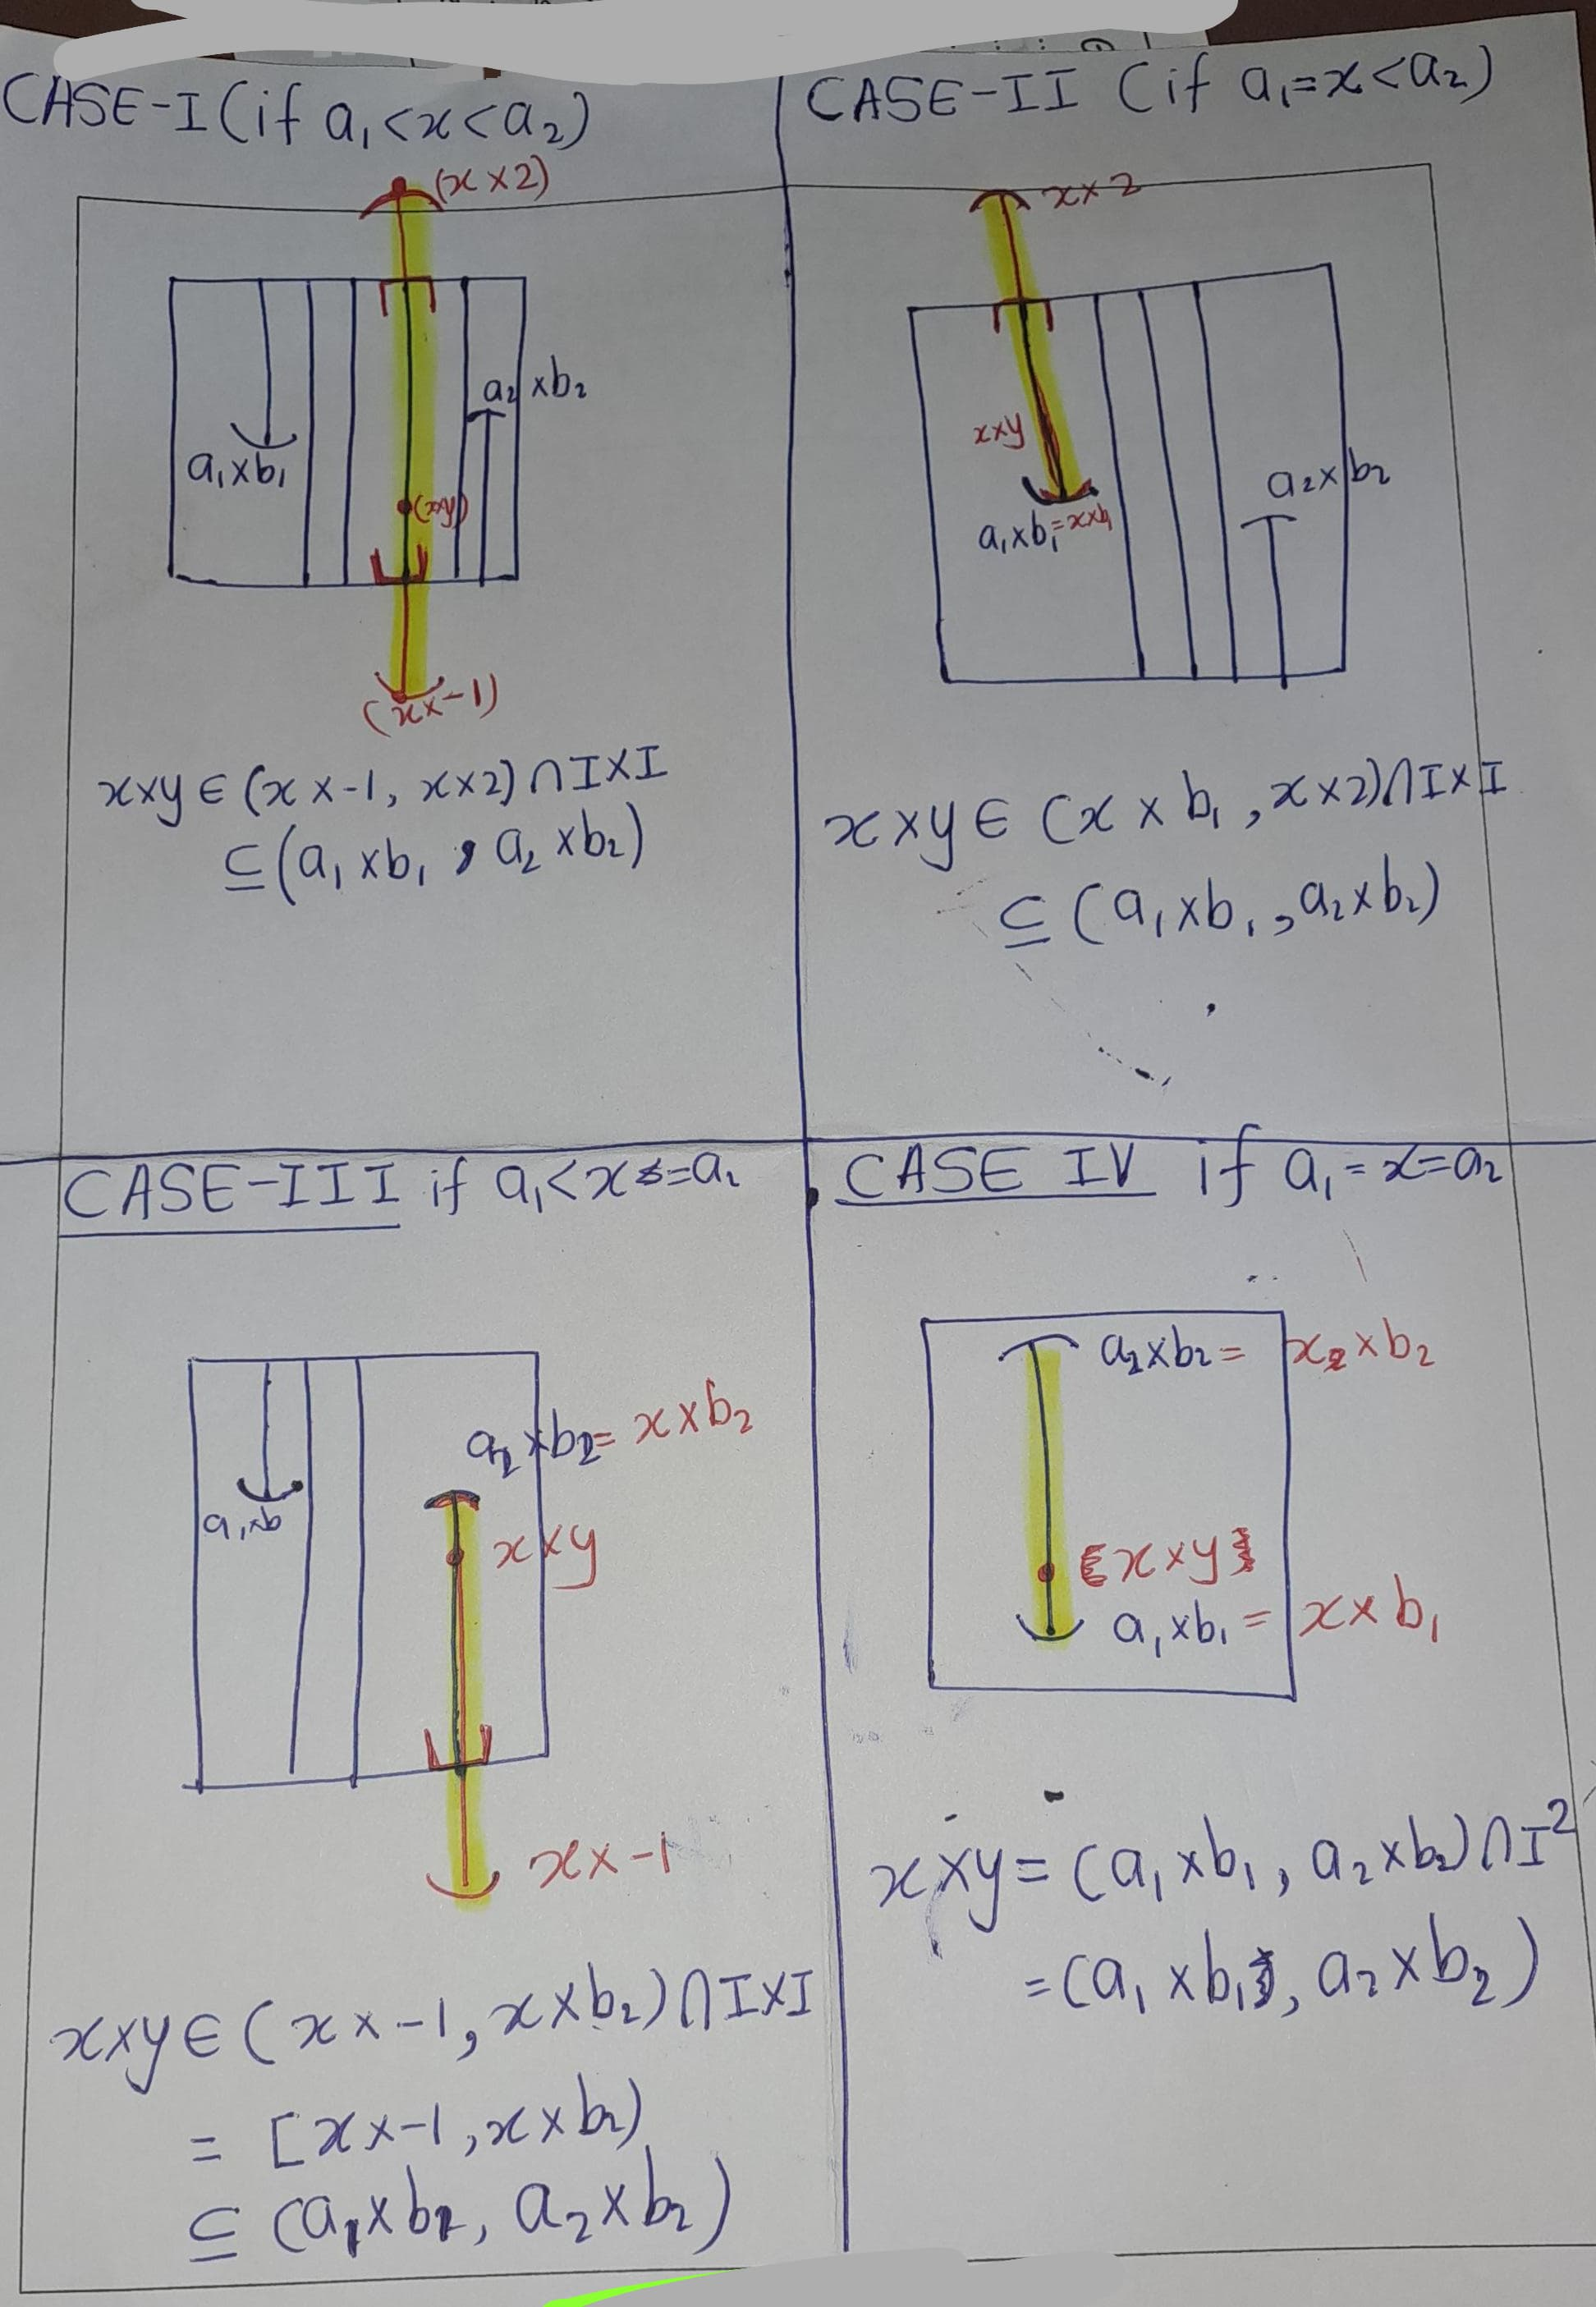
\includegraphics{figures/figure 15.jpg}
\caption{\label{fig:fig15}\(~\)}
\end{figure}

\hypertarget{closed-sets-and-limit-points}{%
\section{Closed Sets and Limit Points}\label{closed-sets-and-limit-points}}

\emph{Closed sets are nothing but complement of open sets. On the other hand, we can also say that open sets are nothing but
complement of closed sets. Thus we can actually use closed sets to define topology, although mathematicians usually use
open sets to define topology.}

\begin{definition}
\protect\hypertarget{def:unnamed-chunk-49}{}\label{def:unnamed-chunk-49}

Let \(A\) be a subset of a topological space \((X, T)\).

\begin{itemize}
\tightlist
\item
  \(A\) is a closed set of \(X\) if \(X - A\) is an open set.
\item
  The closure \(\overline{A}\) of \(A\) in \(X\) is the intersection of all closed sets of \(X\), containing \(A\).
\item
  The interior \(\text{Int}A\) of \(A\) in \(X\) is the union of all open sets of \(X\), contained in \(A\).
\item
  \(x \in X\) is a limit point of \(A\) if \(x \in A\setminus\{x\}\)
\end{itemize}

\end{definition}

\hypertarget{chapter-2-name}{%
\chapter{Chapter 2 name}\label{chapter-2-name}}

\hypertarget{chapter-03-name}{%
\chapter{Chapter 03 name}\label{chapter-03-name}}

Up to there is none.

\hypertarget{exercises}{%
\chapter{Exercises}\label{exercises}}

\hypertarget{exercise-after-section-16-in-munkress-book}{%
\section{Exercise after Section 16 in Munkress Book}\label{exercise-after-section-16-in-munkress-book}}

\begin{exercise}
\protect\hypertarget{exr:unnamed-chunk-50}{}\label{exr:unnamed-chunk-50}Show that if \(Y\) is a subspace of \$X, and \(A\) is a subset of \(Y\) , then the topology \(A\) inherits as a subspace of \(Y\) is the same as the topology it inherits as a subspace of \(X\).
\end{exercise}

\textbf{Solution}:
Let's denote the topology on \(X\) as \(\mathcal{T}_X\), the topology on \(Y\) as \(\mathcal{T}_Y\), and the topology on \(A\) as \(\mathcal{T}_A\).

We know that \(Y\) is a subspace of \(X\), so the topology \(\mathcal{T}_Y\) that \(Y\) inherits from \(X\) is \(\mathcal{T}_Y = \{ Y \cap U : U \in \mathcal{T}_X \}\).

Similarly, \(A\) is a subset of \(Y\), so the topology \(\mathcal{T}_A\) that \(A\) inherits from \(Y\) is \(\mathcal{T}_A = \{ A \cap V : V \in \mathcal{T}_Y \}\).

Substituting \(\mathcal{T}_Y\) into the equation for \(\mathcal{T}_A\), we get \(\mathcal{T}_A = \{ A \cap (Y \cap U) : U \in \mathcal{T}_X \}\).

Since \(A\) is a subset of \(Y\), \(A \cap Y = A\). So, \(\mathcal{T}_A = \{ A \cap U : U \in \mathcal{T}_X \}\).

This is exactly the topology that \(A\) would inherit as a subspace of \(X\). Therefore, the topology \(A\) inherits as a subspace of \(Y\) is the same as the topology it inherits as a subspace of \(X\).

  \bibliography{book.bib,packages.bib}

\end{document}
